\documentclass[12pt,a4paper,oneside]{article}

\usepackage[pdftex,
            pdfauthor={Albert Zak},
            pdftitle={Reactively Querying an Immutable Log of Relational Facts.
            Design and Implementation of a Bitemporal EAV Database with a Subscription Query Language.},
            pdfsubject={Master's Thesis},
            hidelinks,
            driverfallback=hypertex]{hyperref}
\usepackage[english]{babel}
\usepackage{lmodern}
\usepackage[utf8]{inputenc}
\usepackage[T1]{fontenc}
% \usepackage{arialu}
% \renewcommand{\familydefault}{\sfdefault}
% \normalfont
\renewcommand{\rmdefault}{phv} % Arial
\renewcommand{\sfdefault}{phv} % Arial

\usepackage{microtype}
\usepackage{geometry}
\usepackage{bookmark}
\usepackage{listings}
\usepackage[inline]{enumitem}
\usepackage{subcaption}
\usepackage{tabularx}
\usepackage{cleveref}
\usepackage{multirow}
\usepackage{floatrow, makecell}
\usepackage{hhline}
\usepackage{boldline}
\usepackage{algpseudocode}
\usepackage{stackengine}
\usepackage{tikz}
\usetikzlibrary{trees,arrows,fit,positioning,shapes.geometric,shadows}
\PassOptionsToPackage{usenames,dvipsnames,svgnames,table}{xcolor}
\usepackage{xcolor-solarized}
\usepackage{gitdags}
\usepackage[singlespacing]{setspace}
\usepackage[acronym,nopostdot,style=super,nonumberlist,nogroupskip]{glossaries}
\usepackage{fancyhdr}
\usepackage{hyphenat}
\hyphenation{name-space}
\usepackage{forest}
\forestset{
  dir tree/.style={
    for tree={
      parent anchor=south west,
      child anchor=west,
      anchor=mid west,
      inner ysep=-3pt,
      grow'=0,
      align=left,
      edge path={
        \noexpand\path [draw, very thin, lightgray, \forestoption{edge}] (!u.parent anchor) ++(1em,0) |- (.child anchor)\forestoption{edge label};
      },
      font=\ttfamily,
      if n children=0{}{
        delay={
          prepend={[,phantom, calign with current]}
        }
      },
      fit=band,
      before computing xy={
        l=2em
      }
    },
  }
}

\pagestyle{fancy}
\fancyhf{}
\cfoot{\thepage}
\renewcommand{\headrulewidth}{0pt}

\makeglossaries{}
\newacronym{ACID}{ACID}{Atomicity, Consistency, Isolation, Durability}
\newacronym{EAV}{EAV}{Entity-Attribute-Value}
\newacronym{RDBMS}{RDBMS}{Relational Database Management Systems}
\newacronym{tx}{$t_x$}{transaction time}
\newacronym{SPA}{SPA}{Single Page Application}
\newacronym{SQL}{SQL}{Structured Query Language}
\newacronym{tv}{$t_v$}{valid time}
\newacronym{REST}{REST}{Representational State Transfer}
\newacronym{JSON}{JSON}{JavaScript Object Notation}
\newacronym{RDF}{RDF}{Resource Description Framework}
\newacronym{ORM}{ORM}{Object-Relational Mapping}
\newacronym{XML}{XML}{Extensible Markup Language}
\newacronym{RAD}{RAD}{Rapid Application Development}
\newacronym{CRUD}{CRUD}{Create, Read, Update, Delete}
\newacronym{DDD}{DDD}{Domain-Driven Design}
\newacronym{FRP}{FRP}{Functional-Reactive Programming}
\newacronym{SaaS}{SaaS}{Software-as-a-Service}
\newacronym{DDP}{DDP}{Decentralized Data Protocol}
\newacronym{MUMPS}{MUMPS}{Massachusetts General Hospital Utility Multi-Programming System}
\newacronym{edn}{edn}{Extensible Data Notation}
\newacronym{CQRS}{CQRS}{Command Query Responsibility Segregation}
\newacronym{CRDT}{CRDT}{Conflict-free Replicated Data Type}
\newacronym{OT}{OT}{Operational Transform}
\newacronym{lvar}{lvar}{logic variable}
\newacronym{HTTP}{HTTP}{Hypertext Transfer Protocol}
\newacronym{CALM}{CALM}{Consistency as Logical Monotonicity}
\newacronym{IETF}{IETF}{Internet Engineering Task Force}
\newacronym{API}{API}{Application Programming Interface}
\newacronym{CAP}{CAP}{Consistency, Availability, Partition tolerance}
\newacronym{DSL}{DSL}{Domain-specific language}
\newacronym{UI}{UI}{User Interface}
\newacronym{DRP}{DRP}{Distributed Reactive Programming}
\newacronym{6NF}{6NF}{6\textsuperscript{th} normal form}
\newacronym{ES}{ES}{Event Sourcing}
\newacronym{txe}{txe}{Transaction entity}


\lstset{
  language=lisp,
  numbers=left,
  numberstyle=\small\color{lightgray},
  basicstyle=\ttfamily,
  captionpos=b,
  frame=tb,
  extendedchars=true,
  firstnumber=0,
  stepnumber=5,
  xtopmargin=5pt,
  xbottommargin=5pt,
  xleftmargin=17pt,
  framextopmargin=5pt,
  framexleftmargin=17pt,
  framexrightmargin=5pt,
  framexbottommargin=5pt,
  inputencoding=utf8,
  mathescape=true
}
% Hide number in first line of code listings
\makeatletter
\def\lst@PlaceNumber{\ifnum\value{lstnumber}=0\else
  \rlap{\normalfont\kern\linewidth \kern\lst@numbersep\lst@numberstyle{\thelstnumber}}\fi}
\makeatother

\newcommand{\lisp}[1]{\lstinline$#1$}

\pdfpageheight=297mm
\pdfpagewidth=210mm
\geometry{a4paper, left=30mm, right=25mm, top=30mm, bottom=30mm}

\begin{document}

\frenchspacing

\pagestyle{empty}
\thispagestyle{empty}
\begin{picture}(50,50)
  \put(-70,40){\hbox{
\includegraphics[width=5cm]{fhcw-logo.pdf}}}
\end{picture}

\vspace*{-5.8cm}


\begin{center}
  \vspace{6.5cm}
  \hspace*{-1.0cm} {\LARGE \textbf{Reactively Querying an Immutable\\}}
  \hspace*{-1.0cm} {\LARGE \textbf{Log of Relational Facts\\}}
  \vspace{0.5cm}
  \hspace*{-1.0cm}
  Design and Implementation of a Bitemporal

  \hspace*{-1.0cm}
  EAV Database with a Subscription Query Language

  \vspace{1.2cm}

  \hspace*{-1.0cm} {\LARGE \textbf{Master Thesis\\}}
  \vspace{0.65cm}

  \hspace*{-1.0cm} Submitted in partial fulfillment of the requirements for the degree of \\

  \vspace{0.65cm}

  \hspace*{-1.0cm} \textbf{Master of Science in Engineering} \\
  \vspace{0.65cm}
  \hspace*{-1.0cm} to the University of Applied Sciences FH Campus Wien \\
  \vspace{0.4cm}
  \hspace*{-1.0cm} Master Degree Program\\
  \hspace*{-1.0cm} Software Design and Engineering\\

  \vspace{2cm}

  \hspace*{-1.0cm} \textbf{Author:} \\
  \vspace{0.2cm}
  \hspace*{-1.0cm} Albert Zak \\
  \vspace{0.7cm}

  \hspace*{-1.0cm} \textbf{Student identification number:}  \\
  \vspace{0.2cm}
  \hspace*{-1.0cm} 1810838004 \\
  \vspace{0.7cm}

  \hspace*{-1.0cm} \textbf{Supervisor:} \\
  \vspace{0.2cm}
  \hspace*{-1.0cm} Priv.-Doz. Mag.rer.soc.oec.\\
  \hspace*{-1.0cm} Dipl.-Ing. Dipl.-Ing. Dr.techn.\\
  \hspace*{-1.0cm} Karl Michael Göschka \\
  \vspace{0.7cm}

  \hspace*{-1.0cm} \textbf{Date:} \\
  \vspace{0.2cm}
  \hspace*{-1.0cm} 2020-05-31 \\

\end{center}

\newpage

\vspace*{16cm}
\begin{flushleft}
  \underline{Declaration of authorship:}\\
  \vspace{0.5cm}
  I declare that this Master Thesis has been written by myself. I have not used any other than the listed sources, nor have I received any unauthorized help.\\
  \vspace{0.5cm}
  I hereby certify that I have not submitted this Master Thesis in any form (to a reviewer for assessment) either in Austria or abroad.\\
  \vspace{0.5cm}
  Furthermore, I assure that the (printed and electronic) copies I have submitted are identical.\\
  \vspace{1cm}
  Date: \hspace{5.3cm} Signature:
\end{flushleft}


\newpage
\pagestyle{fancy}
\pagenumbering{roman}
\cleardoublepage{}

\section*{Abstract}




\section*{Key Terms}
EAV \\
Database \\
Bitemporal \\
Immutable \\
Datalog \\
Lisp \\

\cleardoublepage

\renewcommand{\glsnamefont}[1]{\textbf{#1}}
\doublespacing
\printglossary[title=List of Abbreviations,nonumberlist,type=\acronymtype]
\singlespacing

\cleardoublepage


\tableofcontents{}

\cleardoublepage

\pagenumbering{arabic}

\section{Introduction}

This thesis describes a possible design and a proof-of-concept implementation of a data layer for near real time distributed collaborative applications targeted at operational workloads in small to medium sized businesses with strict auditability requirements.

\paragraph{Context.} The ideas presented in this work are based on the author's experience running a \gls{SaaS} business developing and operating a highly available information system in the medical sector for the past five years (see~figure~\ref{fig:rosalind}). The deployed system covers all of the daily operational needs of medium-sized practices, handling medical records, personal data, and associated imagery for more than 80.000 patients a year, scheduling appointments, employees, departments, and rooms subject to complex business rules constraining available treatments, forecasting, planning and reporting clinical workload, sending appointment reminders, handling inbound calls and messages from patients, recording internal referrals and escalations, along with support for distributed staff (e.g. external call centers, telemedicine) owing to fine-grained roles and authorization controls, thorough audit logging of all changes, and compliance with relevant regulations.

\begin{figure}[!ht]
  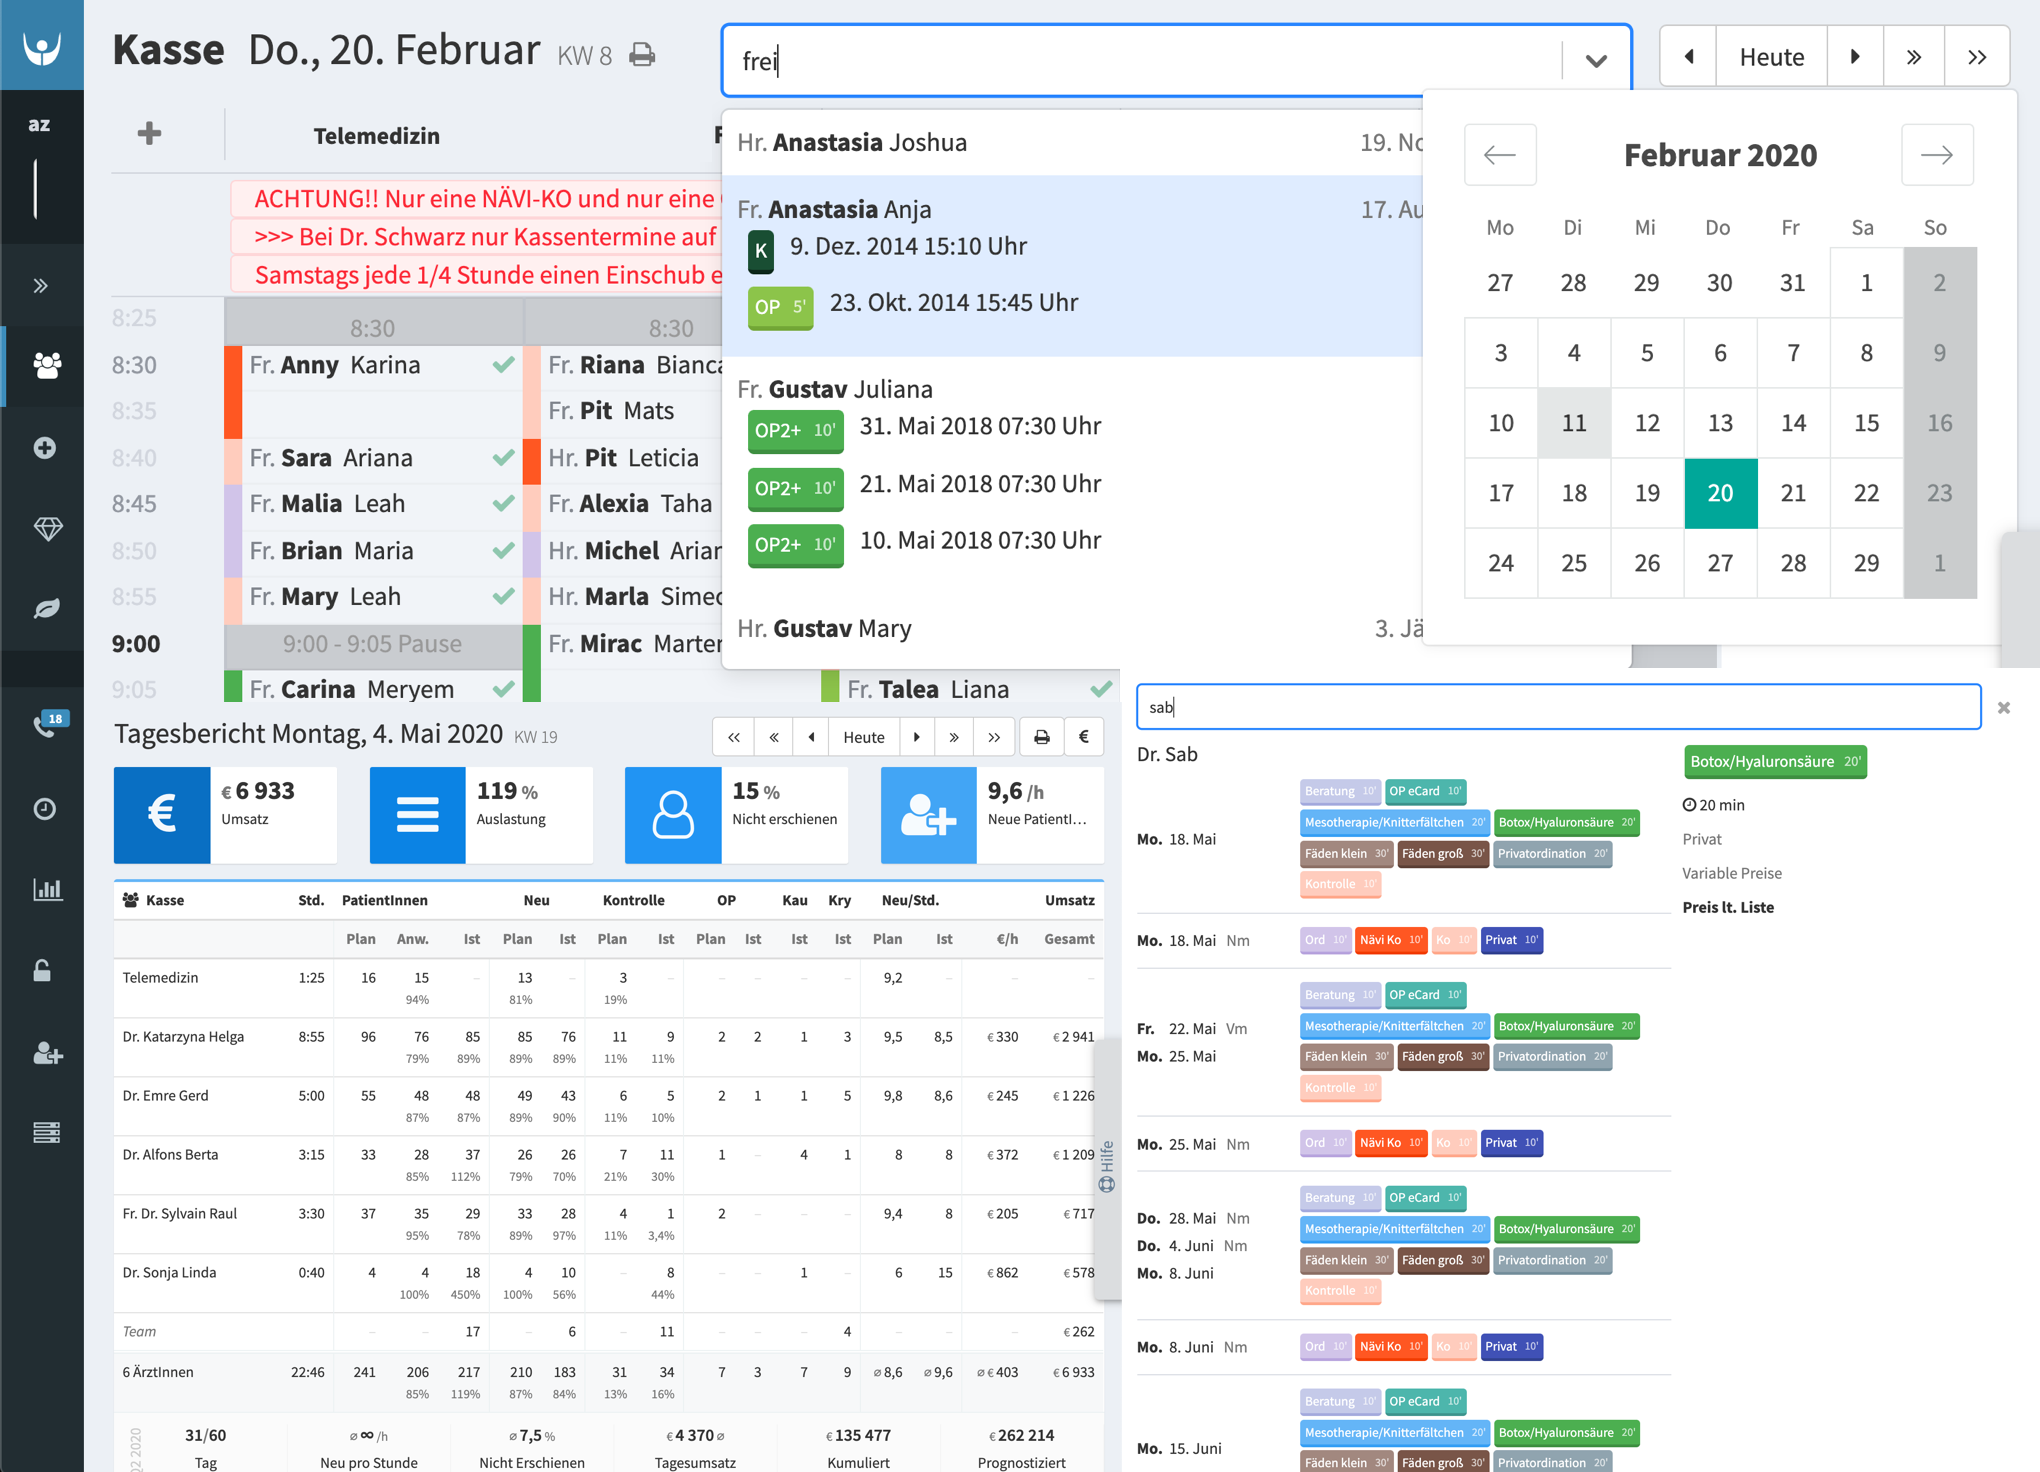
\includegraphics[width=\linewidth]{images/rosalind.png}
  \caption{The author's medical information system}
  \label{fig:rosalind}
\end{figure}


\cleardoublepage

\paragraph{Background.} The system is built on top of the open source Meteor framework (presented in section~\ref{sec:related_work}) and MongoDB, making heavy use of their "live query" mechanisms, along with Redux, React and Minimongo in the front end, packaged with Electron and React Native. To increase availability, the back end is deployed over three data centers using primary-backup replication. Currently, the tracked code base comprises about 42.000 lines of JavaScript. Being a system designed, developed, and operated by a single person, the primary challenge by far has been to keep runaway incidental complexity at bay. While the abstractions around "live" publication/subscription provided by the Meteor framework turned out to be very expressive, other design decisions of the underlying framework and database caused unnecessary complexity in the application code. Drawbacks include pervasive mutability, the need to denormalize data, the lack of a relational query language, no server-side joins, and no (bi-)temporality or notions of time or memory for auditing purposes.


\paragraph{Outline.} Section~\ref{sec:related_work} presents related work. Section~\ref{sec:design} exhibits common problems experienced in data-intensive business applications and shows a different approach towards solving some of them in a functional, immutable, and reactive way. A proof-of-concept implementation is described in section~\ref{sec:implementation} and its merits and deficiencies are discussed in section~\ref{sec:discussion}.

\cleardoublepage

\subsection{Problem}
Classic Relational Database Management Systems (RDBMS) are not suitable for modeling sparse, hierarchical or multi-valued data in domains where evolution and dynamism are hard requirements. They also lack a notion of memory or change over time because writes are destructive by default. Attempts to add concepts of temporality to Structured Query Language (SQL) are complicated and, as a result, not widely used. Auditing changes to a mutable black box with no history is hard. Developers fear the networking aspects of sending queries on a round trip "over there" \cite{hickey2012dbvalue} to the database, as opposed to having the data in memory and being able to query it directly. On top of all, customers demand increasingly interactive distributed collaboration environments, which pushes the limits of established request-response mechanisms.

\subsection{Contribution}
This thesis explains a possible design of a data layer for business applications and describes its prototypal implementation. The core is a simple relational data model based on facts in the form of Entity-Attribute-Value (EAV) tuples similar to the \gls{6NF} or the \gls{RDF} as seen in Semantic Web literature. Such EAV tuples are accreted in an append-only (immutable) log as assertions and retractions together with two timestamps: \gls{tx} at which the fact was added to the log, and \gls{tv} at which the fact became true in the wider context of the system \cite{snodgrass1992temporal} i.e., the real world.


\paragraph{Goal.}
The original goal of this work was to demonstrate the feasibility of an implementation of various desirable data layer features in less than 1000 lines total of readily comprehensible Lisp (Clojure, more specifically ClojureScript \cite{hickey2008clojure}): Bitemporality, practically immutable audit logging, transaction metadata, server-client reactivity, schemalessness, consistency criteria, derived facts, versatile indexing, transactions with guarantees of \gls{ACID}, and a simple relational query language based on Datalog.

\paragraph{Method.}
The thesis explains the decisions made while iterating on the design and its implementation and includes a discussion on limitations and advantages.

\paragraph{Results.}
Embracing the EAV+$t_x$+$t_v$ data model together with the expressive programming language ClojureScript reveals that it is possible to implement a proof-of-concept data layer and query language for business applications with various valuable features not commonly seen in mainstream databases. The implementation is realized using less than 400 lines of code, the majority of which appears to map fairly well to the conceptual design.

\subsection{State of the art}\label{sec:sota}

The system presented in this thesis builds on various ideas around better ways of dealing with of data, state, and process in distributed information systems.

\paragraph{Entity-Attribute-Value (EAV).}

Representing information in \emph{attribute-value pairs} dates back to Lisp from the late 1950s \cite{mccarthy1960recursive}. Together with a value identifying the \emph{entity}, the EAV data model is able to represent arbitrary data in a single table of just three columns (and many rows) by forcing normalization to the 6\textsuperscript{th} normal form (6NF). The basic unit of information in EAV systems is the \emph{fact}, which is a triple \lisp{[e a v]} consisting of:

\begin{enumerate}[nolistsep,label={(\roman*)}]
  \item \lisp{e}, a value identifying the \emph{entity} to which the fact is related,
  \item \lisp{a}, an \emph{attribute} value, and
  \item \lisp{v}, the \emph{value} itself.
\end{enumerate}

The EAV data model is also known as \emph{open schema}, or \emph{vertical database} \cite{jastrow2015entity}. Medical information systems TMR \cite{stead1983chartless} and HELP \cite{huff1994help} were the first to bring this way of knowledge representation to a clinical context in the 1970s. EAV later gained popularity through the Semantic Web and the Resource Description Framework (RDF) \cite{decker2000semantic} where facts are called object-attribute-value triplets. In domains where the number of attributes related to an entity is large and modeling such data in a classical \gls{RDBMS} would require dealing with the overhead of defining and storing many columns, the EAV model provides an efficient and simple way to deal with sparse data.

\begin{lstlisting}[label={lst:examplefacts},morekeywords={patient,name,room,building},caption=A sequence of EAV facts]
[[:patient/91 :name "Hye-mi"]
 [:patient/91 :room :room/32]
 [:room/32 :building "A-12"]
 ...]
\end{lstlisting}

While all \emph{current} state of the system can be represented conceptually as in listing~\ref{lst:examplefacts} as a single (long) sequence of facts, it would be useful to know exactly \emph{how} the system got into its current state.


\paragraph{Logs.} 16\textsuperscript{th} century seafarers invented the \emph{log} \cite{may1973historylog}. With a piece of wood -- the log -- attached to a string and thrown into the water, they could track its speed relative to the ship over time and record the measurements in a logbook, along with other events of interest \cite{kakkar19log}.

In data-intensive applications, the log is today often treated as a side product of mutating central state in a database, to aid in understanding situations after something has gone wrong. However, ideas such as \gls{ES} have reversed the roles of log and database and dictate that state is inferred from an accretion of events.

\cleardoublepage
\paragraph{Event Sourcing.} Systems which derive their state by consuming an ordered sequence of events are called \emph{event sourced}. In practice, event sourcing is commonly associated with, and used in conjunction with \gls{DDD} \cite{evans2004domain} and the architectural pattern of \gls{CQRS} \cite{kabbedijk2012case}.

DDD tends to be employed in domains where the shape of the data is mostly known in advance and generally remains rather static over the lifetime of the system, because domain events are generally tied to the code because they are modeled as classes closed for modification.

CQRS is an architectural separation of the read paths from the write paths. In the case of classic event sourcing, this implies that when new data comes in as part of an event, the event is first appended to the global log. Afterwards, one or more materialized views (in a regular RDBMS) are updated from which the application finally performs its reads, as reading from  the unwieldy log directly would be inefficient and complicated, yet such a decoupling of concerns begets additional complexity in application code because read-after-write consistency is not guaranteed.

\paragraph{Immutability.} Tying these ideas together with the EAV data model yields an event sourced database, where events are the most granular write operations on each field, akin to the transaction log of a classical database. To better convey the immutability of the log, the terms \emph{assertion} and \emph{retraction} are used in place of creation and deletion. To change a fact, one issues a transaction which simultaneously retracts the previous value and asserts the new one. An immutable EAV database consequently is the accretion of assertions and retractions of facts over time.

\paragraph{Value orientation.} Instead of thinking about the database as a "place" where to send queries to fetch data from and write data to, the idea pioneered by Datomic is that the entire state of the database at any given point in time should be an \emph{immutable value} which can be passed around in the program. Because it is immutable and a local value, it never changes, implying that subsequent queries on the same value always result in the same results thus giving a \emph{stable basis}.

\cleardoublepage
\paragraph{(Bi-)temporality.}

When extending EAV databases and the idea of \gls{ES} with a first-class concept of time and/or transactions, such systems are sometimes referred to using the ambiguous abbreviation \emph{EAVT}, with the \emph{T} variously referring to either the addition of transaction time, valid time or other \emph{domain time} values (or a combination thereof) \cite{huser2013desiderata} or the \emph{T} may hint at the concept of first-class transactions, where a fact additionally carries the entity ID of its originating transaction to allow attaching arbitrary metadata to events. Listing~\ref{lst:examplefactstx} shows a fact with a pointer to a \emph{transaction entity}, about which bitemporal and other transaction metadata exists as first-class facts. This example demonstrates that the patient was actually ($t_v$) moved to room \#32 at 18:30, but the fact was recorded in the system ($t_x$) later at 21:12 by user \#43 as part of transaction \#4.

\begin{lstlisting}[label={lst:examplefactstx},morekeywords={:tx-id/4},caption=Transaction metadata are first-class facts]
  [[:patient/91 :room :room/32 :txe/4]
   [:tx-id/4 :$t_v$ #inst "2019-05-31T18:30:00"]
   [:tx-id/4 :$t_x$ #inst "2019-05-31T21:12:00"]
   [:tx-id/4 :tx-by :user/43]
   ...]
  \end{lstlisting}

While uni- or monotemporal databases allow querying along the transactional sequence of historic database states (called \gls{tx}), support for bitemporality adds another separate time axis \gls{tv} denoting the time at which the fact came into existence in the wider \emph{context} of the system. Note the there is no limit on the storage of arbitrary additional time-related facts related to an entity or a first-class transaction, the collection of which are referred to as \emph{domain time} facts. A (bi-)temporal database only provides efficient and convenient indexing and query capabilities for $t_x$ and $t_v$ values. Users querying for any other values -- including domain time -- must use the general querying mechanisms.

\paragraph{\gls{FRP}.}
Conceived initially to describe graphical animations \cite{elliott1997functional}, the FRP paradigm applies nicely to distributed data-intensive systems where it yields composable building blocks which are relatively easy to reason about \cite{reynders2014multi}.

FRP fits particularly well inside the view layer of a \gls{SPA} to construct the view out of (nested) pure functions $v=f(s)$ which take a global state value and return a description of what to render. Each component function specifies what slice of the state it needs, recursively composes smaller components, and is automatically re-run when the state changes.

Apart from web development, \cite{salvaneschi2013towards} gives an overview of the literature on the more general \gls{DRP} paradigm.


\cleardoublepage
\paragraph{Distributing state.} The complexity of state within a single program pales in comparison to the challenges faced when distributing said state over the network. The fundamental impossibility of simultaneously honoring all three guarantees of Brewer's conjecture: consistency, availability, and partition-tolerance (CAP) \cite{brewer2000towards} later proven by \cite{gilbert2002brewer} implies -- in the case of a network partition, because networks can and will fail (with partition being a particularly nasty failure) -- write or read semantics to be either "pessimistic" yet safe and consistent (but blocked until the partition is healed) yielding CP semantics, or "optimistic" yet possibly resulting in inconsistencies that, in the case of writes, need to be reconciled later (but remaining available for reads and/or writes) resulting in AP behavior. A real-world network is asynchronous, thus even in case of no partitions, there exists a tradeoff between latency and availability, as captured by Abadi's \gls{PACELC} \cite{abadi2012consistency} formulation: In case of partitions, choose between availability and consistency, else -- meaning during normal operation -- trade between latency and consistency. Note that these tradeoffs do not globally apply to the system as a whole, but are to be separately decided for each data item and each type of action.

This work argues in favor of a more fine-grained and far-reaching distribution of state throughout the layers of a distributed application, particularly towards clients keeping a queryable slice of the state in memory, somewhat similar to \cite{jungnickel2018feasibility} but lacks the strong guarantees of convergence as provided by e.g. Conflict-free replicated data types (CRDTs), yet at least brings auditable structured bitemporal history of all changes.

\cleardoublepage
\section{Related Work}\label{sec:related_work}

\paragraph{\gls{RAD}.} Scaling developer productivity as the team size goes $n \to 1$ on data-intensive near real time collaborative line-of-business applications goes back to the \gls{RAD} movement of the 1990s sparked by tools such as the Delphi suite \cite{mackay2000reconfiguring}, PowerBuilder \cite{zubeck1997implementing}, Lotus Notes \cite{zubeck1997implementing}, and FileMaker
\cite{chen2010developing}.

\paragraph{MUMPS.} On the aspects of near real time state synchronization combined with RAD tooling, a notable mention is the \gls{MUMPS} \cite{bowie1979methods} dating back to the year 1966. An extremely terse programming language combined with a runtime system featuring built-in persistence mechanisms. Its "global database" is a subscripted array which replicates and persists \emph{code and data} across machines in near real time. Major hospitals and financial institutions continue to run their daily operational workloads on various evolutions of MUMPS systems today \cite{aller2018evolution}.

\paragraph{Firebase et al.} Firebase and Parse are hosted services which brought real time state synchronization to web and mobile applications starting in 2011. Firebase is a proprietary managed service operated by Google. Its data model is based on a global mutable structure in \gls{JSON} and allows only rather simplistic filtering and navigational queries \cite{wingerath2019real}. Parse was a similar real time Backend-as-a-Service based on MongoDB and Redis which was active from 2011 to 2017. An open source client-side database which allows subscribing to the result set of a query is RxDB for JavaScript replicating PouchDB, CouchDB, or GraphQL endpoints \cite{wingerath2019real}. The data model of these services is generally oriented around mutable documents in free-form nested \gls{JSON}, although there are means to validate records via a schema.


\paragraph{Meteor.} This thesis is an evolution based on the author's experience running a \gls{SaaS} business built on the Meteor \cite{schmidt2014live} framework and the \gls{DDP} \cite{ddpspec} which were released in 2012. Meteor allows clients to transparently subscribe to the results of predefined MongoDB queries updating live over arbitrary durations. Synchronization is achieved by the server watching the operations log of the database (called "oplog tailing") \cite{wingerath2019real}, keeping track of the entire set of published documents and subscribed queries for each connected client, and computing delta changes to send back to the client. See table \ref{tbl:dbcomparison} for a comparison of Meteor with other data management approaches.

Clients cache the received documents in a local instance of MongoDB implemented in JavaScript (called Minimongo), enabling local queries with no latency via an API that mostly mirrors the server-side MongoDB interface. Combined with a functional-reactive view library such as React to bind the management of a view's lifecycle with its data subscriptions, this setup gives the impression of data "just being here" on the client with almost no programmatic overhead.

\cleardoublepage
Reads are by default served from the client's local copy of the data, giving an AP read path that may result in the reading of stale data but remains performant and available. The application developer can choose to apply writes either optimistically to the local database which Meteor later replicates to the server (that may issue corrections) thus yielding AP characteristics with last-write-wins pseudo resolution semantics (previous writes are lost because there is no concept of time); or let the server process the transaction via a Remote Procedure Call (RPC) and wait for a quorum of the database servers before confirming and replicating to the clients, thus yielding CP semantics.

The major problem of Meteor is its absolute dependence on MongoDB and the ensuing lack of a relational data model, i.e. no joins and requiring to denormalize data, leading to incidental complexity of the application code and the $n+1$ query problem. Its Minimongo implementation lacks indices and does not support all of MongoDB's query capabilities. Meteor's publication/subscription mechanism does not scale well to many clients or publication queries returning a large number of documents. This is because the server keeps a working copy of all documents present in each connected client's local database in memory and creates a diff for each client on each database update. As a result, Meteor's publication/subscription mechanism is stateful and requires sticky sessions, meaning that an upstream load balancer must take care to always forward a client's requests to the same backend server.

Preliminary load testing and tracing of performance problems during typical workloads encountered in the author's medical information system concluded that performance of Meteor's publication/subscription system starts to degrade noticeably with more than 300 clients connected to one server process on moderate dedicated server hardware, or when a client subscribes to a single publication containing more than around 100,000 documents. Clients subscribing to such large collections has intermittently led to server processes permanently hanging at 100\% processor usage until forcibly restarted, an issue which has been known for at least two years\footnote{Meteor issue \#9796 on GitHub: \url{https://github.com/meteor/meteor/issues/9796}}. Despite these shortfalls, Meteor is production-grade software with extraordinary developer ergonomics and served as the backbone of the authors's business replicating terabytes of data extremely reliably since first put into production five years ago.

While this work originally aimed to design a publication/subscription mechanism with developer usability goals similar to Meteor's, its focus shifted towards an exploration of a wholly different data layer based on a model implementation of an immutable bitemporal EAV database, with only minimal yet general query subscription capabilities remaining.


\begin{table}[]
  \caption{Comparison of Meteor with other database and stream processing systems \cite{wingerathcase}}
  \begin{tabular}{r|c|c|c|c|}
    \cline{2-5}
                                              & \textbf{DBMS}                                                & \textbf{\begin{tabular}[c]{@{}c@{}}Real-time\\ database\end{tabular}}            & \textbf{\begin{tabular}[c]{@{}c@{}}Data stream\\ management\end{tabular}} & \textbf{\begin{tabular}[c]{@{}c@{}}Stream\\ processing\end{tabular}}     \\ \hline
    \multicolumn{1}{|r|}{\textbf{data}}       & \multicolumn{2}{c|}{\begin{tabular}[c]{@{}c@{}}persistent\\ collections\end{tabular}}                                                           & \multicolumn{2}{c|}{\begin{tabular}[c]{@{}c@{}}persistent \& ephemeral\\ streams\end{tabular}}                                                       \\ \hline
    \multicolumn{1}{|r|}{\textbf{processing}} & one-time                                                     & \begin{tabular}[c]{@{}c@{}}one-time \&\\ continuous\end{tabular}                 & \multicolumn{2}{c|}{continuous}                                                                                                                      \\ \hline
    \multicolumn{1}{|r|}{\textbf{access}}     & random                                                       & \begin{tabular}[c]{@{}c@{}}random \&\\ sequential\end{tabular}                   & \multicolumn{2}{c|}{sequential}                                                                                                                      \\ \hline
    \multicolumn{1}{|r|}{\textbf{streams}}    & \multicolumn{3}{c|}{structured}                                                                                                                                                                                             & \begin{tabular}[c]{@{}c@{}}structured \&\\ unstructured\end{tabular}     \\ \hline
    \multicolumn{1}{l|}{}                     & \begin{tabular}[c]{@{}c@{}}PostgreSQL,\\ MongoDB\end{tabular} & \begin{tabular}[c]{@{}c@{}}Firebase,\\ Meteor,\\ RethinkDB,\\ Parse\end{tabular} & \begin{tabular}[c]{@{}c@{}}Influx,\\ PipelineDB,\\ SQLStream\end{tabular} & \begin{tabular}[c]{@{}c@{}}Storm,\\ Samza,\\ Flink,\\ Spark\end{tabular} \\ \cline{2-5}
    \end{tabular}
    \label{tbl:dbcomparison}
  \end{table}

\paragraph{Datomic.} Most of the design tenets for the project described in section~\ref{sec:design} originate from the database Datomic \cite{hickey2012dbvalue} which was created by the author of the Clojure programming language in 2012. Its data model is a monotemporal (transaction time \gls{tx} only) and immutable log of assertions and retractions of EAV facts, with first-class transactions being reified as regular queryable facts themselves. Datomic requires a minimal schema to be specified upfront.

Instead of thinking of the database as a single \emph{place} to send queries to and receive tuples from, Datomic separates its components as follows to achieve horizontal read scalability, turning the classical model of a database "inside out" \cite{kleppmann2017designing}:
\begin{itemize}
  \item There is a \emph{generic} stateful distributed storage layer, which may be backed by any pluggable implementation (SQL, Redis, Riak, Kafka, files, memory...). The storage layer keeps all data in the form of tuples and various indices. \cite{hickey2019datomic}.
  \item Application servers (called "peers") operate on a working set of tuples in memory. They perform queries themselves \emph{locally on their own copy of the data.} Tuples are cached locally as needed and are lazily loaded from the storage layer over the (local) network, where disk locality is considered irrelevant \cite{ananthanarayanan2011disk}. As put by the author: "perception does not require coordination \cite{hickey2012values}", yet consistency and caching are trivial because tuples are immutable.
  \item All write transactions -- represented as data structures -- go through a \emph{single} instance of the \emph{transactor} component, which is the only part of the system that may write to the storage backend. Because it is one single threaded instance, it can impose a global order on all incoming transactions. Conversely, the transactor is the bottleneck for write throughput, as well as a single point of failure for which a second instance should be operated in a hot failover configuration. Peers can place first-class functions into the database, and call them as part of a transaction to enforce arbitrary data invariants \cite{datomicdocs}.
\end{itemize}


\paragraph{Crux.} Rooted in the same core principles as Datomic but having taken some different architectural choices, Crux is an efficient \emph{bitemporal} schemaless unbundled document database. For a detailed comparison with Datomic, see \cite{juxtcrux}.

\cleardoublepage

\paragraph{Datascript et al.} Similarly inspired by Datomic, DataScript \cite{prokopov15datascript} is an immutable schemaless in-memory EAV store. It lacks notion of time and history because it is designed to manage frequently changing client-side state of an \gls{SPA} within the browser for the lifetime of a session where memory is limited.

Several attempts exist, including this thesis, to bridge the gap between a Datomic-like database on the server and a DataScript-like instance on the client, which may be used simultaneously for client-only view state as well as for caching tuples from the server \cite{small16datscript}; and for closing the gap between that database and the view layer \cite{parker15posh,krivosheev19reposh}. Datahike \cite{datahike} is a port of DataScript back to the server, where it adds durable persistence. It aims to be a single-node replacement for Datomic suitable for use in small projects.

Mozilla Mentat \cite{mozillamentat} was an attempt at a performant embeddable implementation in Rust of a combination of ideas from Datomic, DataScript, and SQLite.

Eva \cite{eva} is an open source monotemporal EAV database very similar to and compatible with the \gls{API} of Datomic, though the project appears to be abandoned in a feature-complete "alpha" quality stage.

Ittyon \cite{ittyon} is a Clojure library to manage distributed state in games based on ideas from Entity-Component Systems (ECS) combined with the EAV+$t_x$ data model. The testbed described in section~\ref{sec:implementation} is based on its client/server implementation.

This thesis takes ideas related to increased expressivity from each of these projects and presents a greatly simplified implementation which ignores all aspects of performance, efficiency, or interoperability.

\paragraph{Hyperfiddle, LogicBlox, and Eve.} A notable proprietary commercial RAD self-serve database system with an integrated programming language based on Datalog, LogicBlox \cite{aref2015design} similarly aims to reduce incidental complexity of developing line-of-business applications with a focus on probabilistic and predictive analytics of large business data sets. Its developers have contributed a novel efficient algorithm for incremental view maintenance for Datalog systems \cite{veldhuizen2012leapfrog}.

The ongoing Hyperfiddle project \cite{getz18hyperfiddle} aims to be a \gls{DSL} to fully describe an application using only plain expressions of \gls{edn}. It is built on Datomic to interactively and quickly create a \gls{UI} for database applications,

Ambitious but ultimately abandoned, the Eve project \cite{eve} was an attempt to reinvent programming for "humans first" through a combination of development environment, database, and a novel relational and reactive programming language where e.g. the concept of identifier scope is abandoned, and the order of statements has no semantics.

If the data layer presented in this thesis would be evolved towards a full framework for declaratively turning business requirements into functioning applications, following in the spirit of Meteor, the resulting product could look like a combination of Hyperfiddle, LogicBlox and Eve.

\section{Design}\label{sec:design}

The contribution of this work is divided into two main sections, design and implementation. The subsequent parts of this section first present various design problems of commonly employed data layer technologies. Deriving from their limitations, the next part paints a blissful picture of what an ideal data layer would look like (subsection~\ref{sec:goals}), while the following demarcates the scope of the contribution (subsection~\ref{sec:nongoals}). Finally, the conceptual model (subsection~\ref{sec:conceptual_model}) and the query language (subsection~\ref{sec:query_language}) are presented.

\subsection{Problems}

Traditional RDBMSs enforce a structural rigidity of fitting data into "tables", "rows", and "columns", entailing a lack of flexibility in dealing with sparse data, irregular data, hierarchies, or multi-valued attributes \cite{hickey2012dbvalue}. With the shift to data-intensive Single-Page Applications (SPAs), clients become limited peers to the database. Requirements of real time collaboration, evolution of the schema, and auditability of changes, together with limited request-response data loading mechanisms work together to increase the incidental complexity of application code.


\paragraph{\gls{SQL}.}
Despite the widespread use of SQL, it is not, in any version, an accurate reflection of the relational model \cite{codd1990relational} \cite{tarpit}.
Modeling domains in common \gls{RDBMS} requires distinguishing between entity and relationship \cite{chen1976entity}. A system in which choosing the structure for the data involves setting up "routes" between data instances (such as from a particular employee to a particular department) is access path dependent. A pure relational systems would need no problematic distinction between entity and relationship \cite{tarpit}.

SQL within the application's main programming language is usually treated as a second class citizen by resorting to concatenation of strings with a thin layer of sanitization. (Microsoft's LINQ \cite{meijer2006linq} is a notable exception.) Features such as materialized views are cumbersome to use because the language lacks powerful means of abstraction and composition \cite{sicp} which would enable recursively composing complex queries out of smaller queries.

\paragraph{Object-relational mismatch.}
\gls{ORM} of tuples from the database onto whichever data types are available in the backend programming languages, and increasingly also to the language in the front end in \gls{SPA}, as well as the choice of appropriate communication interfaces between at least three layers pose additional considerations. Duplicating structure in schema definitions and again in ORM code leads to a proliferation of types.

\paragraph{Time.}
Temporal databases are commonly optimized for analytics performance over large numeric datasets, e.g. sensor readings over time. Temporal extensions to SQL \cite{kulkarni2012temporal} are convoluted and do not address the fundamental problem at hand, which is that typical mutable-state systems obscure the sequence of events that brought the world into its current state.

\paragraph{Distribution.}
Thinking that data resides "over there" on a remote server breeds a "fear of round trips" and causes developers to accumulate incidental complexity in the form of performance optimizations related to caching \cite{hickey2012dbvalue}.

Yet, one cannot disavow the fundamental complexities of distributed systems: Network failures (latency, disconnection, offline context), consistency and availability choices taken by underlying technology which are not made explicit, and how different representations of data influence and determine what is and is not possible in terms of concurrent activity by different actors \cite{emerick2014api}.

\paragraph{Imperative fetching.}
Performing data loads via classic request-response semantics is not expressive enough because the act of fetching is made explicit and requires imperative calls to various endpoints. A developer of a \gls{SPA} with a \gls{REST} backend must decide along which boundaries to split the data endpoints. In traditional RESTful style, each \emph{resource} dictates its own endpoint with its own \gls{CRUD} actions. This approach places the burden of orchestrating a decomposed rich interaction on the clients \cite{calderwood15cqrs}, leading to the $n+1$ query problem when performing client-side joins, and an over-fetching of data which is not needed to display but happens to be provided by the endpoint.

At the other extreme, there exists one distinct endpoint providing the exact required data for each screen (notwithstanding that the concept of a \emph{screen} is vague in SPAs) which collects, filters, and joins the data on the server before serializing it as one tree, and sending it back to the client. This style causes incidental complexity through a proliferation of endpoints and ad-hoc schemata.

A middle-ground mixture of both styles is common, muddling the architectural waters and bringing both disadvantages together with even more code bloat. In any case, the act of fetching the data must be initiated by the client in an imperative way instead of data just being "here" in the client's view layer when needed.


\paragraph{Propagation of updates.}
The traditional understanding of queries for data at rest as in listing~\ref{lst:querying_data_at_rest} is that data exists at the database in one place, and queries are passed over there, usually in the form of SQL strings, and unroll themselves into a dataflow tree of operators, pulling data up the tree when they reach the leaves \cite{alvaro2015isee}.

\begin{lstlisting}[label={lst:querying_data_at_rest},morekeywords={employees,departments},caption=Querying data at rest \cite{alvaro2015isee}]
($\Pi$ [:name :department]
   ($\bowtie$ ($\sigma$ :name "Scott" employees)
      departments))
\end{lstlisting}

When the underlying data changes, queries do not get re-run automatically and clients are left looking at stale data. On the flip side, re-running the same query at different times is not guaranteed to yield the same results, as the database might have changed in the mean time. There are no facilities to temporally stabilize a basis for queries.

\subsection{Goals}

a flexible \emph{data layer} for small to medium size internal business applications for distributed collaboration in near-realtime.
out of the author's experience running a SaaS business designing, developing, and operating a
why no there are many special purpose dbs, mostly for performance.
but none optimized for "data just being there when you need it"

with least amount of code. but still backed by relational guarantees (acid)

needs different kind of db.
needs reinvention of the whole data layer.



To reduce some of the complexities in question, moseley and Marks recommend adopting functional and declarative programming constructs, along with a fully relational data model \cite{tarpit}.

\paragraph{Streaming relational queries.}
Recall the querying semantics for data at rest in \autoref{lst:querying_data_at_rest}. What is needed for rich interactions is a different model of streaming queries for data in motion: What is "just there" is not the data, but the query — which is \emph{instantiated in the network}, and the data flows through the query instead of the other way around. \autoref{lst:querying_data_in_motion} gives an example of a streaming query.

\begin{lstlisting}[label={lst:querying_data_in_motion},morekeywords={email-source,contacts-source},caption=Querying data in motion \cite{alvaro2015isee}]
($\Pi$ [:ip]
   ($\bowtie$ ($\sigma$ (classifier email :spam)
         email-source)
       contacts-source))
\end{lstlisting}




\paragraph{Notion of memory.}
with strict auditability (log+queryable past)
free auditing of everything, time travel
"save everything", query later
6NF EAV "Event Sourcing" Data Model w/ Explicit Time and Memory: "History of structured Facts"

\paragraph{Transactional guarantees.}
Transactions (ACID)


\paragraph{Adaptivity and dynamism.}
schemaless


\paragraph{Distribution.}
The handling of data between clients and servers should be as declarative as possible: Clients declare what data they are interested in, and the infrastrucutre takes care of fetching, caching, handling updates, unsubscribe

Isomorphic + Homoiconic: Single Language: ClojureScript on Lumo/Browser




`'\subsection{Non-goals}\label{sec:nongoals}


\paragraph{Efficiency.}
No attention is paid to the efficiency of compute and memory usage. Tradeoffs are almost always made in favor of clarity concerning the mapping between conceptual model and implementation of the proof of concept. The only major optimization is the fact that the triple index structure exists, leastwise it doubles as the simplest possible way to access arbitrary data without the overhead of parsing and executing a query.

Custom indexing strategies, e.g. ways to maintain a phonetic index to query for people's names, do not need to be part of the database design, because the triple indexing scheme is general enough to allow arbitrary access to the data in a manner that is efficient enough without having to declare indices upfront.

\paragraph{First class bitemporality.}
Another non-goal is the efficiency, primacy, and expressive power of the provided bitemporal affordances. A vast amount of previous work exists on relatively complex attempts to add efficient bitemporal semantics to relational databases \cite{snodgrass1996adding,jensen1999temporal,kulkarni2012temporal} notably for use in bitemporal constraints \cite{doucet1997using} or within complex queries, and of bitemporality as a first class concept in production rule systems \cite{aref2015design}. Bitemporality in the described system is only secondary. Access paths are optimized for the most recent view of the data, while bitemporality is meant to be used for infrequent auditing purposes. There is no bitemporal index, consequently issuing queries with temporal modifiers causes a sequential scan of the log.

\paragraph{Standard protocols.}
Lastly, the design explicitly avoids compliance with existing proliferated standards around the handling of data such as SQL, \gls{XML}, \gls{JSON}, \gls{REST}, etc. to instead allow quick exploration into different paradigms unburdened by past decisions.



\subsection{Conceptual model}\label{sec:conceptual_model}

The data model of the presented system is extremely simple. There is no requirement to design a schema or to differentiate between entities and relationships. Yet, \emph{all} structured data can be represented in the system as long as data is fully normalized (6NF).

\begin{itemize}
  \item The basic unit of information is a \emph{fact}, a triple \lisp{[e a v]} containing values representing \emph{entity}, \emph{attribute}, and \emph{value}.

  \item Over time, facts are \emph{asserted} and \emph{retracted}, accreted as part of a \emph{transaction}.

  \item The database and all changes to its state over time are fully described by the transaction log of assertions and retractions of facts.
\end{itemize}

\paragraph{Indexing.}

EAV systems commonly keep a number of sorted indices (see table \ref{tbl:indices}) to allow the data to be retrieved from multiple "angles" or directions, depending on the need of the query. Index structures are named after the \emph{nesting order} in which the elements of the facts are arranged. Not all database systems maintain the same indices. In this case, the system keeps four indices covering the following common use cases:
\begin{itemize}
  \item EAVT, the canonical order, which \emph{maps} an entity to its attributes like a document,
  \item AEVT, for finding entities which \emph{have} a certain attribute set
  \item AVET, for \emph{filtering} entities by a known attribute set to a known value,
  \item VAET, for \emph{searching} over all attributes of all entities by a known value.
\end{itemize}


\newcolumntype{s}{>{\hsize=.5\hsize}X}

\begin{table}[]
  \caption{Impact of the index sort order on the area of application}
  \begin{tabularx}{\textwidth}{|l|s|s|X|}
  \hline
  \textbf{index} & \textbf{name}               & \textbf{feels like}      & \textbf{good for}                                     \\ \hline
  EAVT          & "entity-oriented"           & document store           & accessing various attributes of a known entity        \\ \hline
  AEVT          & "attribute-entity-oriented" & column store             & accessing the same attribute of various entities      \\ \hline
  AVET          & "attribute-value-oriented"  & filtering a column store & finding entities by the value of a specific attribute \\ \hline
  VAET          & "value-oriented"            & searching everything     & searching over all values, regardless of attribute    \\ \hline
  \end{tabularx}
  \label{tbl:indices}
\end{table}

For example, here is a simple example to pull out the name of a known patient, using only the \lisp{get-in} function of the Clojure core library on the \lisp{:eavt} index:

\begin{center}
  \lisp{(get-in db [:eavt :patient/91 :name])}
\end{center}

One can also leave out the attribute, and get back a map (as a conceptual \emph{document}) containing all known attributes related to that entity.

\begin{center}
  \lisp{(get-in db [:eavt :patient/91])}
\end{center}

Performing a search by name over all patients is similarly trivial using the \lisp{:avet} index, with the result

\begin{center}
  \lisp{(get-in db [:avet :name "Hye-mi"])}
\end{center}


\cleardoublepage
\subsection{Query language}\label{sec:query_language}

The query language of the system is a greatly simplified language modeled after the pattern matching relational query language used in Datomic, which is in turn a Lisp variant of the Datalog \cite{abiteboul1988datalog} language expressed in of Clojure's \gls{edn}.

The choice of language is arbitrary -- any relational language would suffice -- and the core of the database does not depend on any query language capabilities Modeling the language after the one used in Datomic was chosen because not only has the edn notation become a de-facto standard for other EAV databases like Crux, EVA, and Datascript, but because the shape of each query clause maps naturally to the representation of a fact in canonical EAV order.

See listing~\ref{lst:example_query} for an query consisting of four query clauses (the \lisp{:where} part) performing an implicit join, and a final projection (\lisp{:find}) to extract the values bound to the \emph{\gls{lvar}} symbols \lisp{?name} and \lisp{?location}. For example, the query clause \lisp{[?p :name ?name]} applied to the fact \lisp{[:person/123 :name "Hye-mi"]} would result in \emph{binding} the lvar \lisp{?p} to the value \lisp{:person/123}, and the lvar \lisp{?name} to the value \lisp{"Hye-mi"}. Other clauses are bound likewise. Note that multiple occurrences of the same lvar prompt \emph{unification} with the same value, creating an implicit \emph{join}. The order of the query clauses has no semantic meaning.

Performing a query entails applying the \lisp{q} function to a database value and a query. Clients can thus decide whether to leverage the query language via loading a library, or just access the data via the index structures directly.

\begin{lstlisting}[label={lst:example_query},caption="Who from Ulsan is working for whom?"]
'[:find [?name ?company]
  :where [[?p :works-for ?e]
          [?e :name ?company]
          [?p :name ?name]
          [?p :location "Ulsan"]]]
\end{lstlisting}

\paragraph{Temporal and bitemporal queries.}
As stated in section~\ref{sec:nongoals}, the (bi-)temporal aspects of the described system are secondary -- they are to be used for infrequent auditing purposes. Consequently, the design of the indexing and query mechanisms can be greatly simplified be forgoing bitemporal indexing strategies such as \cite{nascimento1995ivtt}.

As the query function simply takes a database as a \emph{value}, a \emph{filtering function} can be applied to the database beforehand. The \lisp{keep} function in listing~\ref{lst:queryfilter} returns a structurally shared and lazy copy of the database filtered by arbitrary bounds of the relevant timestamps $t_x$ and $t_v$.

\begin{lstlisting}[label={lst:queryfilter},caption=Applying a temporal filter before querying,morekeywords={keep,q,<,>}]
  (q (keep
       ($\lambda$ [$t_x$ $t_v$]
         (and (> $t_v$ 300) (< $t_v$ 500)
              (< $t_x$ 700)))
       db) query)
  \end{lstlisting}


\paragraph{Per-entity history.} A common use case in auditing is to retrieve the \emph{history} of all attributes related to a given entity over time. The \lisp{history} function takes a database value (optionally composed with a filtering function as described above) and an entity value, and returns an ordered slice of the log with transactions relevant to the requested entity. Note that it does not make sense to create a new database value from a history log, because that would just result in only the latest values being present in the index yet again.


\paragraph{Publication and subscription}

One of the goals states that clients should be able to declaratively subscribe to the \emph{live result set} of a query. The results and the query itself will change over the duration of a client's session. Each change triggers an immediate re-render of the UI. Conceptually, clients \emph{install} their \emph{subscription queries} on the server, and the infrastructure will re-run the subscription query whenever the underlying data changes and notify the client of the changed results. The design does not prescribe whether or not to replicate past (i.e., superseded or retracted) facts, thus greatly simplifying the proof-of-concept implementation by deferring concerns such as diffing, authorization, and the decision of what exactly to replicate to the clients to the developer customizing this data layer to their use case.

\paragraph{Security.} While extreme dynamism may be warranted in a high-trust environment, a real-world application may interact with some malicious entities and thus needs a means to restrict queries on the server side. In a real-world application, clients would need to authenticate themselves and the server would authorize publication based on access rules. Yet, there is no simple way to statically analyze queries submitted by the client for safety properties, but the server can control which facts are allowed to be replicated to a client. A publication might, for example, choose to not replicate facts with specific attributes, or transform facts to censor parts of the value.

\section{Implementation}\label{sec:implementation}

The following subsections describe the implementation of the design explained in the previous section. The conceptual data model from section~\ref{sec:conceptual_model} is translated to Clojure in section~\ref{sec:impl_datamodel}. Next, a guided tour follows the \emph{data path} from a new fact originating on a client all the way through the server and to the other clients, showing and explaining the simple functions that transform it along the way.


\begin{figure}[!ht]
  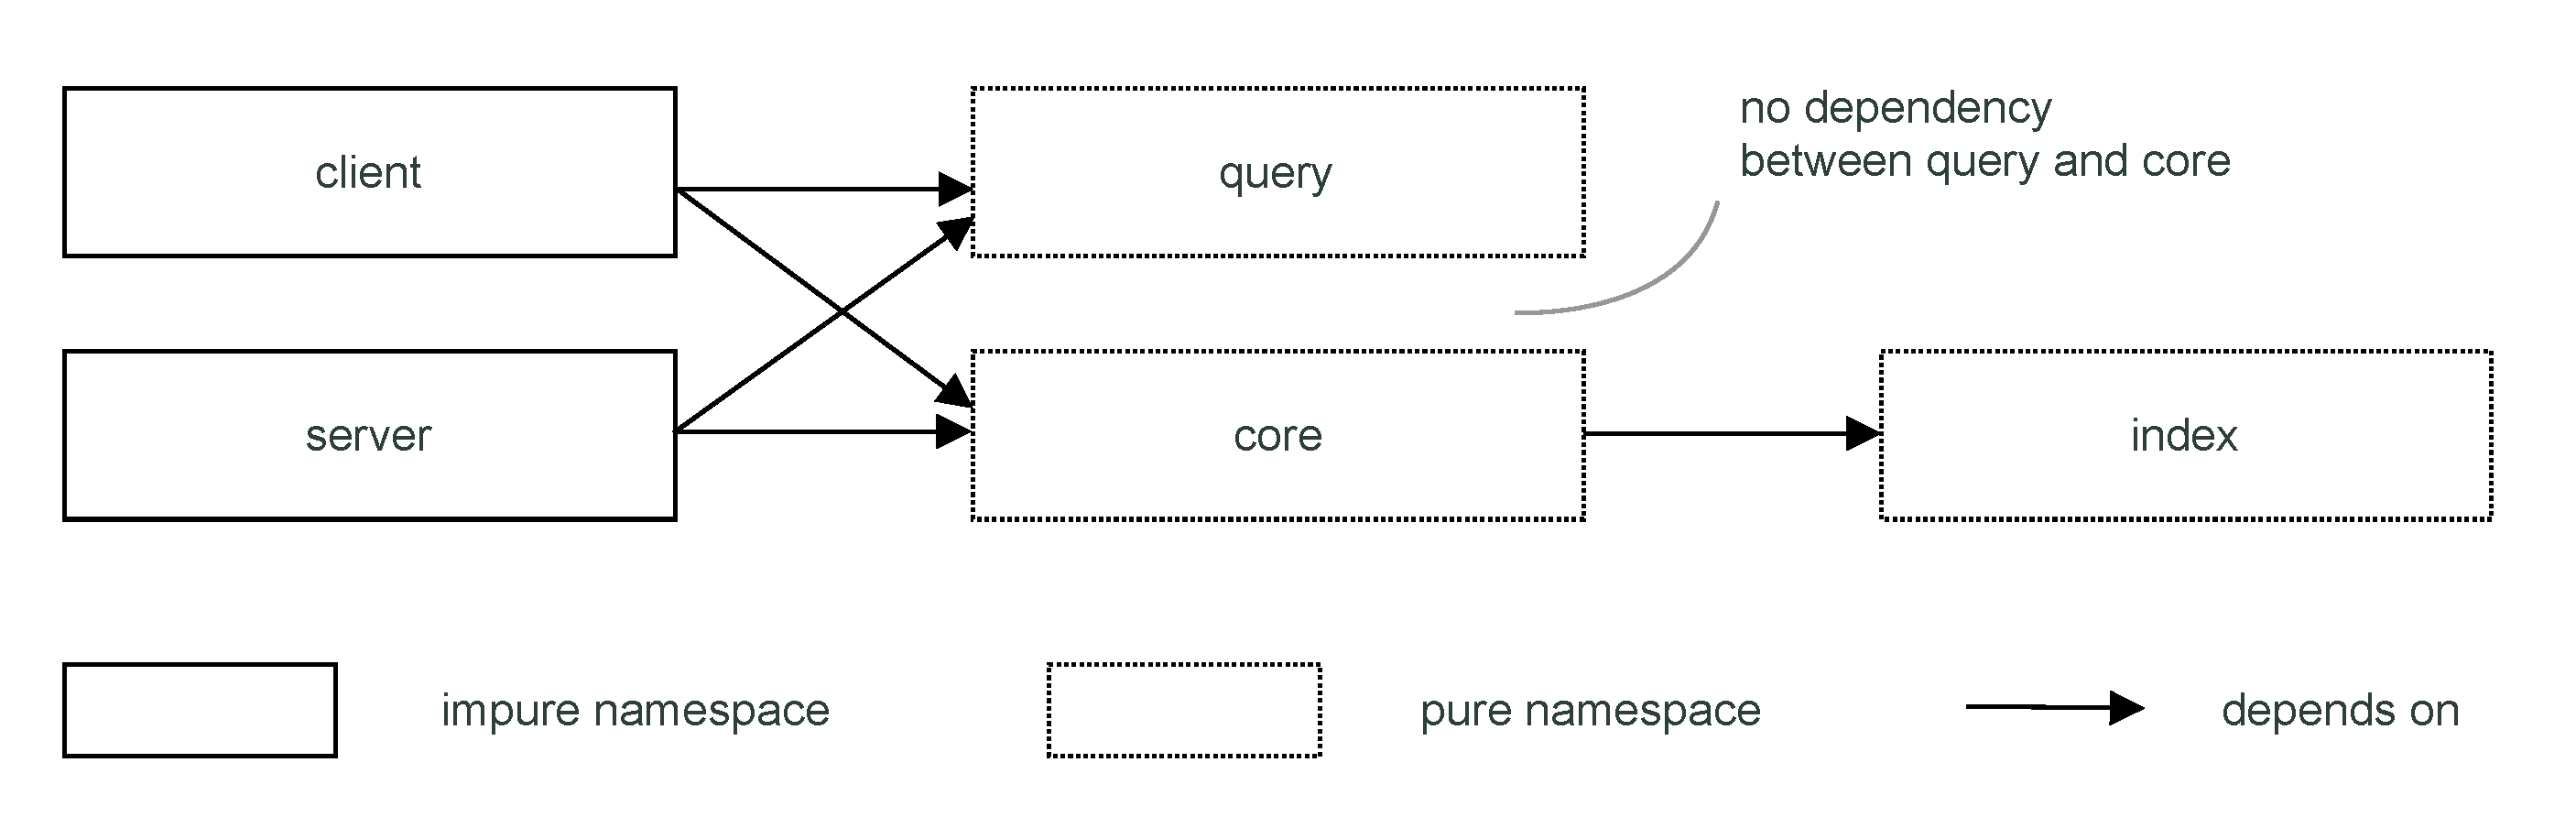
\includegraphics[width=\linewidth]{images/namespaces.pdf}
  \caption{Structure of namespaces}
  \label{fig:namespaces}
\end{figure}


\paragraph{Functional core, stateful shell.}
While Clojure does not enforce functional purity, it is idiomatic to push impure computation and state towards the edge of the system. In fact, core functionality described in the next subsection is implemented as pure functions operating on plain immutable data structures. Such purity allows the same core of the database to run unmodified on servers and on clients. Clients and server obviously need to keep some state, but each does so within one single place only. Three pure namespaces (figure~\ref{fig:namespaces}) make up the functional core of the system:

\begin{enumerate}[label={(\roman*)}]
  \item \lisp{core} implementing the basic pure functions and data structures to create and transact facts,
  \item \lisp{index} implementing pure functions to place facts into indices,
  \item \lisp{query} implementing pure functions to provide basic querying capabilities with a language based on edn Datalog.
\end{enumerate}

The minimal impure parts stay within the \lisp{client} and \lisp{server} namespaces. Their task is to handle the asynchronous connection with each other (\lisp{connect!}, \lisp{disconnect!}, \lisp{receive}, \lisp{broadcast!}) and mutate their local copy of the database (\lisp{transact!})


\cleardoublepage
\begin{figure}[!ht]
  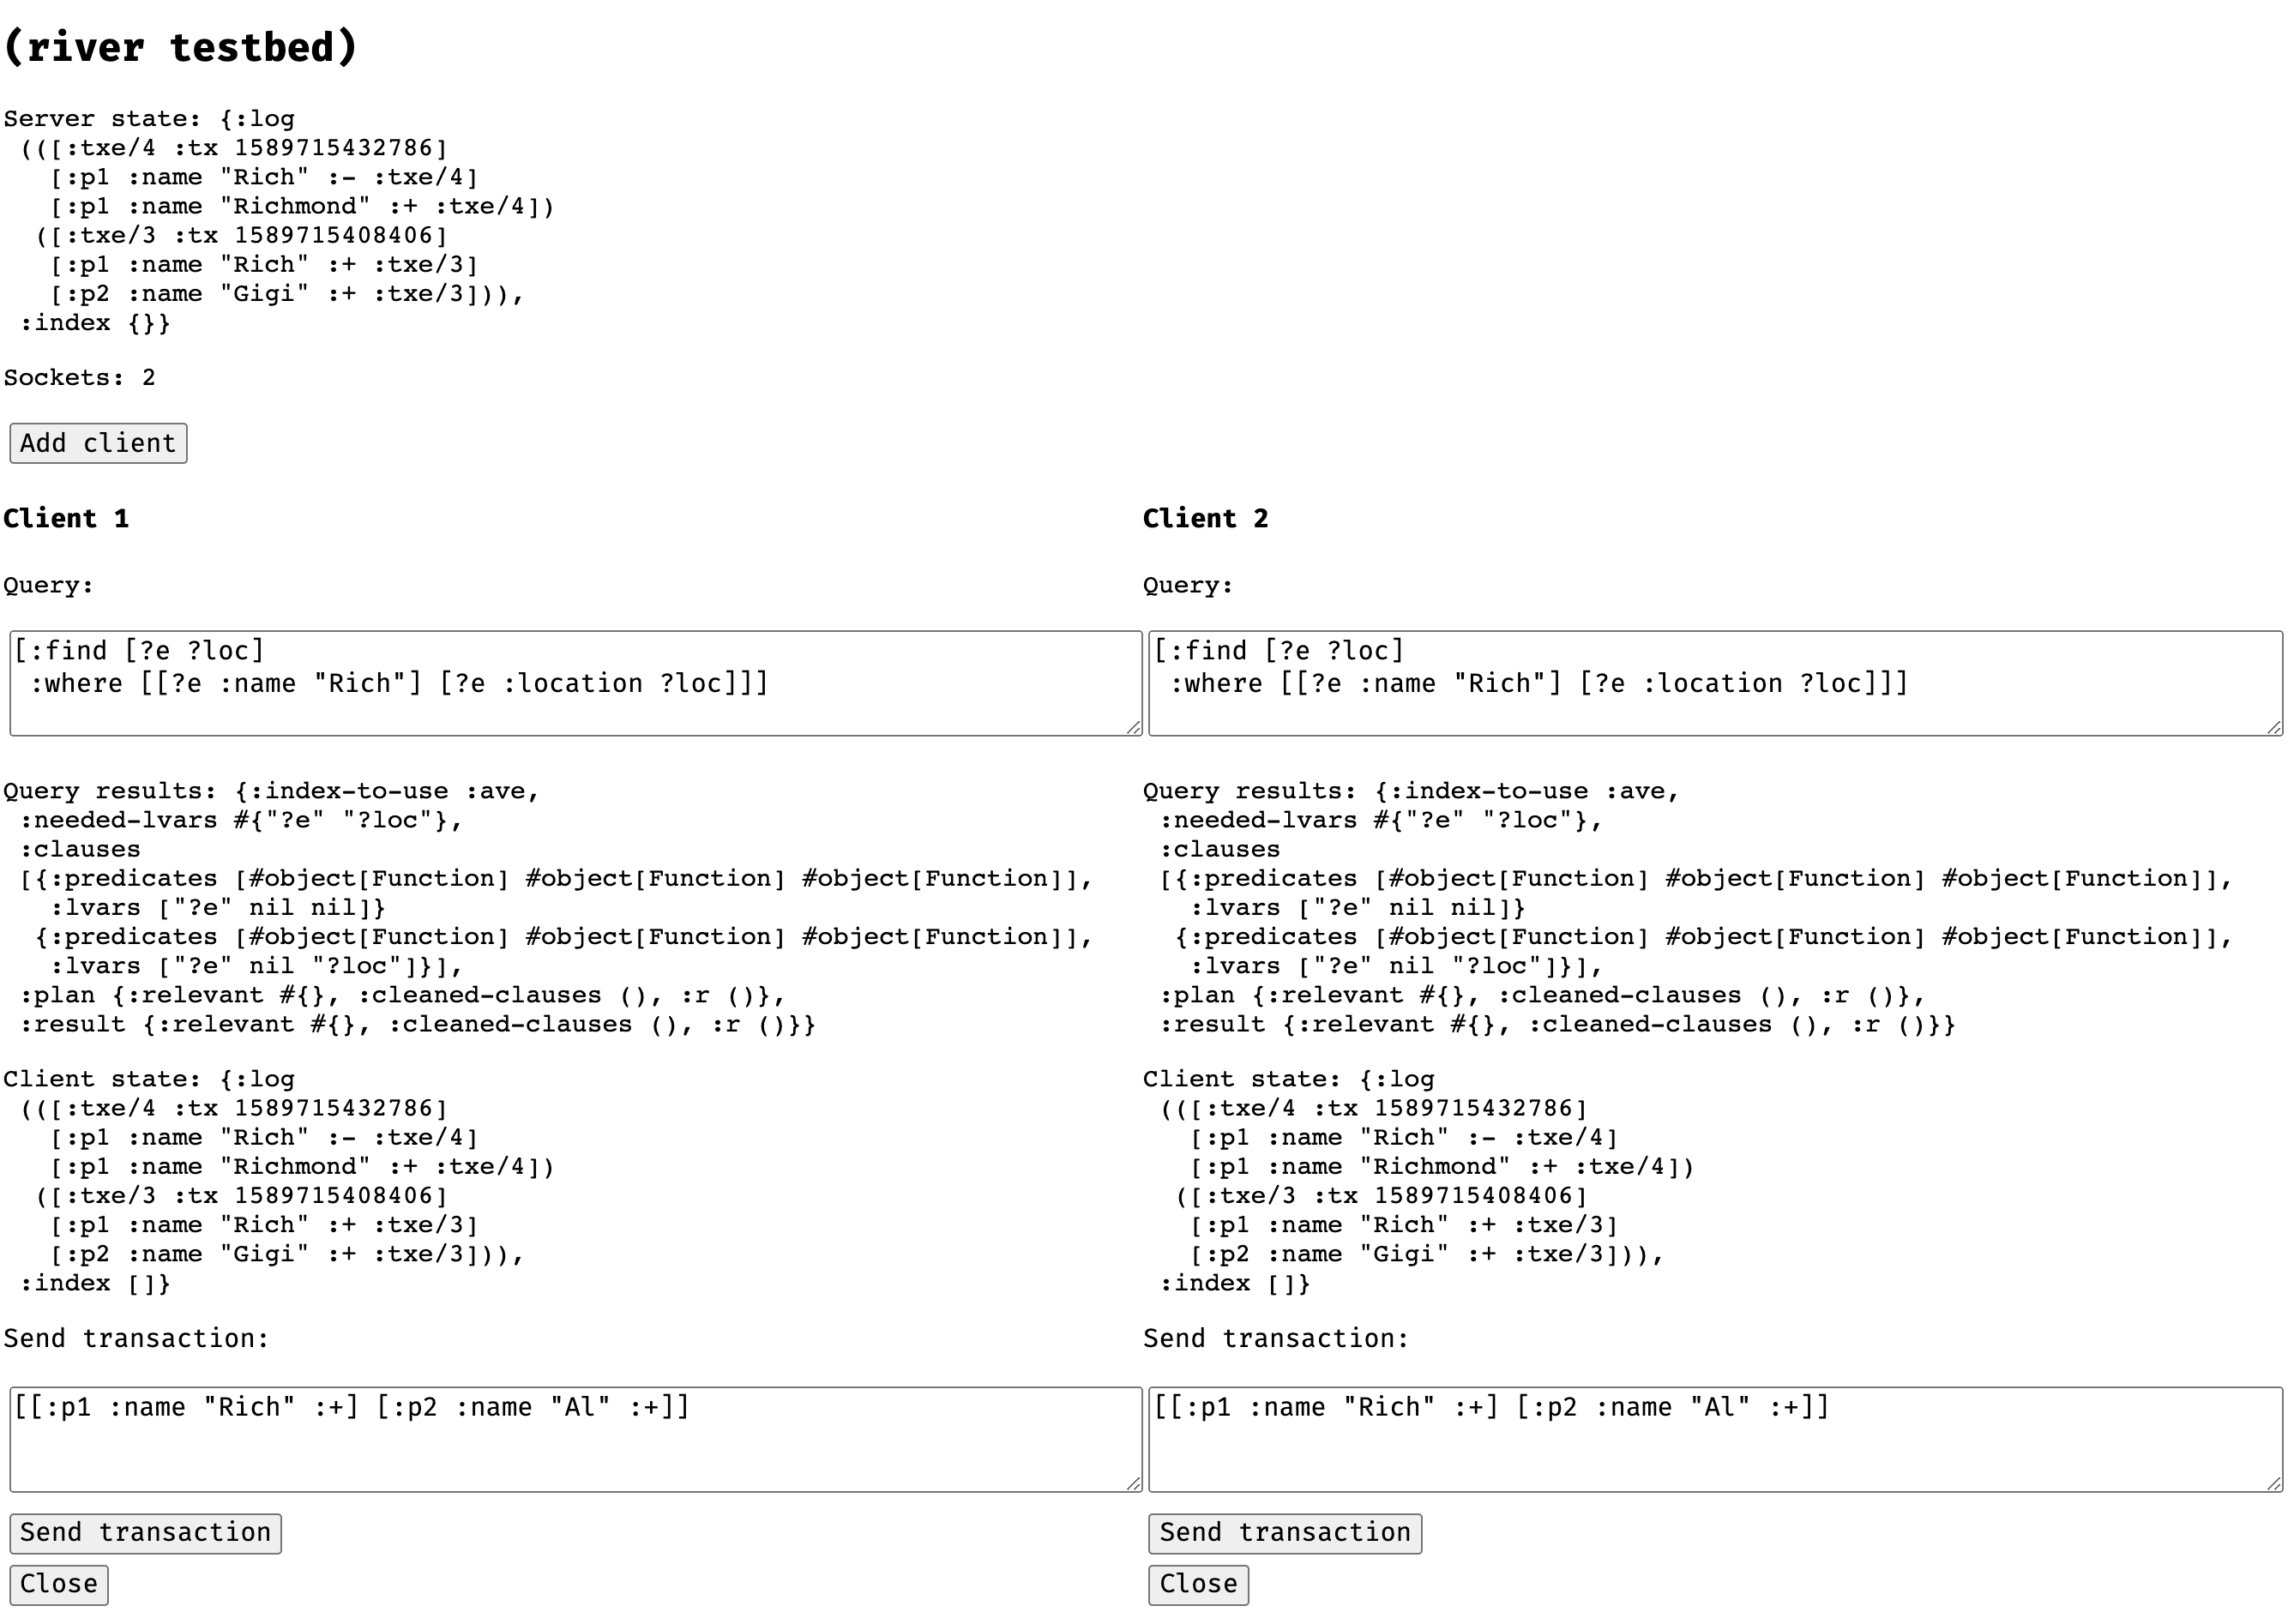
\includegraphics[width=\linewidth]{images/testbed.png}
  \caption{Two connected clients in the testbed}
  \label{fig:testbed}
\end{figure}

\paragraph{The testbed.} To aid quick experimentation while developing, all interactions between the server and the clients are simulated within a single web page. The scaffolding in the \lisp{testbed} namespace presents a simple UI to add and remove client connections, to transact facts, and to perform queries, all while providing insight into the full current state of each simulated node, see figure~\ref{fig:testbed}. The testbed can inject arbitrary delay into Clojure's \lisp{core.async} \emph{channels} used to simulate WebSocket connections between nodes. The channels implementation of the testbed is based on \cite{ittyon}.


\cleardoublepage

\subsection{Data model}\label{sec:impl_datamodel}
The implementation relies heavily on the lazy immutable default data structures \cite{hickey2009persistent} provided by the Clojure core library, which remain performant even when used in strange ways thanks to structural sharing \cite{okasaki1999purely}. This section extends and clarifies the design from section~\ref{sec:conceptual_model} and translates it into Clojure.

\begin{itemize}
\item A \emph{fact} is represented as a vector, its elements can be of any Clojure value type.

\begin{center}
  \lisp{[e a v]}
\end{center}

\item A \emph{transition} is either an \emph{assertion} or \emph{retraction}, a vector containing the splatted fact as its first three elements, along with an indicator whether to assert (\lisp{:+}) or retract (\lisp{:-}) the preceding fact.

\begin{center}
  \lisp{[e a v :+]}
\end{center}

\item A \emph{transaction} is a vector containing an arbitrary number of transitions, which are to be atomically applied to the log \emph{at some point in the future.} Note that a transaction does not mutate the database, it is at this point just a data structure expressing intent to assert or retract facts. A transaction may contain \emph{meta facts} about itself, using the "magic" placeholder value for the transaction entity \lisp{:tx-meta}.

\begin{center}
  \lisp{[[e a v :-] [e a v :+] [:tx-meta a v :+]]}
\end{center}


\item A \emph{commit} (listing~\ref{lst:commit_structure}) is a transaction that was successfully applied to the database, meaning that any consistency criteria succeeded and a new database value containing the updated state was produced. It has similar shape and contents as the transaction it represents. Each transition of the committed transaction contains as its last element the same newly-generated transaction entity reference \lisp{txe}. There is also now at least the $t_x$ transaction meta fact added and optionally any derived facts.

\begin{lstlisting}[label={lst:commit_structure},morekeywords={:+,:-,txe},caption=Structure of a commit]
  [[e a v :+ txe]
   [e a v :- txe]
   [txe :$t_x$ $t_x$ :+ txe]]
\end{lstlisting}

\item The \emph{log} is an ordered linked list of all commits. All changes over time to the database are fully described by the log, with the newest commit being appended to the beginning: \lisp{'([...] [...] ...)}.

\cleardoublepage
\item An \emph{index} (listing~\ref{lst:index_structure}) is an associative nested structure (map). There are four indices, each three layers deep: \lisp{:eavt}, \lisp{:veat}, \lisp{:avet}, named after the nesting order of their keys with the last \lisp{t} referring to the transaction entity \lisp{txe}.

\begin{lstlisting}[label={lst:index_structure},morekeywords={:+,:-,txe},caption=Structure of the indices]
{:index
  {:eavt {e {a {v txe}}
          e {a {v txe}} ...}
   :aevt {a {e {v txe}}
          a {e {v txe}} ...}
   :avet {a {v {e txe}}
          a {v {e txe}} ...}
   :vaet {v {a {e txe}}
          v {a {e txe}} ...}}}
\end{lstlisting}

\item Finally, the \emph{database} (db) is a map containing the log list and the index map (figure~\ref{fig:dbvalue}).

\begin{center}
  \lisp{\{:log '() :index \{\}\}}
\end{center}

\end{itemize}




\begin{figure}[!ht]
  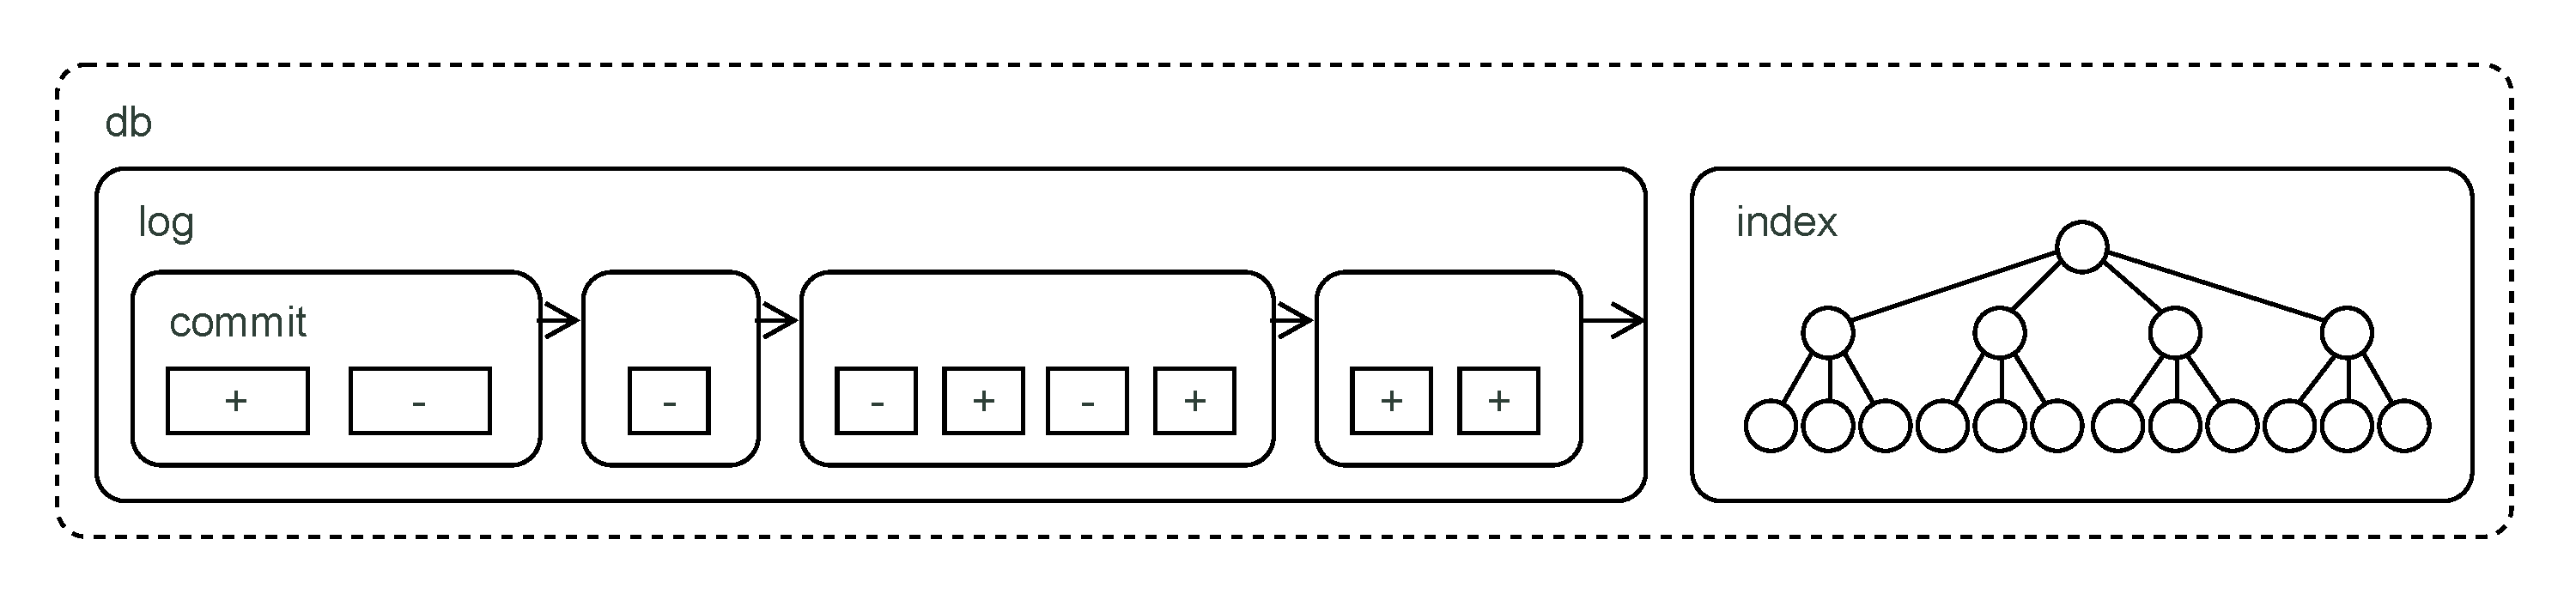
\includegraphics[width=\linewidth]{images/dbvalue.pdf}
  \caption{The database is a value containing the log and the indices}
  \label{fig:dbvalue}
\end{figure}



\paragraph{Commits do not mutate the database.}
Note that a commit itself has no notion of place or state, and does not mutate anything, it only signifies that a transaction was successfully applied to \emph{some} database value \emph{somewhere}. A commit \emph{may} mean that the server has successfully updated its state and broadcast the commit to all connected clients, or, since the database value is immutable, it may just be the result of any local \emph{"as-if"} dry run.

\paragraph{Transaction meta facts.}
A client may supply arbitrary transaction metadata, except $t_x$ which is always set by the server. To send metadata, the client adds transitions to the transaction, which have the magic value \lisp{:tx-meta} set as their entity. Before committing a transaction, the server will replace this value in the transitions with a newly generated entity.

\cleardoublepage
\subsection{Writing}

This subsection follows a simple fact in canonical EAV format, originating on a client, through its transformations until it ends up on the server's canonical source-of-truth database. Starting with the fact

\begin{center}
  \lisp{[:patient/91 :name "Hye-mi"]}
\end{center}

and calling \lisp{assert} on it yields an \emph{assertion transition}, which is created through \emph{conjoining} (appending as last element) the \lisp{:+} keyword with the fact vector. Similarly, calling \lisp{(retract fact)} conjoins \lisp{:-}. The result, the example case, is an assertion vector:

\begin{center}
  \lisp{[:patient/91 :name "Hye-mi" :+]}
\end{center}

The database only accepts transitions to be atomically applied as part of a transaction vector. For example, to update a value, simultaneously retract the previous value and assert a new value for the same combination of entity. The variadic \lisp{transact} function only applies its arguments to \lisp{vector}, creating a transaction vector:

\begin{center}
  \lisp{[[:patient/91 :name "Hye-min" :-] [:patient/91 :name "Hye-mi"  :+]]}
\end{center}

\paragraph{On cardinalities.} What would happen if one were to assert multiple values for the same combination of entity and attribute? Should any previous values be retracted automatically, resulting in one value being "true" at a time? Should all values stay current until retracted? The path chosen in this implementation was to only support the more general case of \emph{defaulting to multi-valued cardinalities on all attributes} (which also happens to be simpler to implement). This may lead to unexpected results in queries. A production system would need to define a schema and enforce cardinalities of \emph{many} or \emph{one} on each attribute depending on the requirements of the domain model.

\paragraph{Server interface.}
This transaction can now be committed to a database value, either locally to create a new database (sometimes also referred to as a "what-if" transaction, as it does not affect the value on the server), or globally for all clients by transacting on the server. In production systems, a server should likely not accept arbitrary transactions from clients. Instead, the database is protected by regular \gls{RPC} / REST endpoints which, after authentication, authorization, and sanitization accept only specific parameters to transact.

The testbed server accepts one type of message, a vector beginning with the keyword \lisp{:transact} containing the entire transaction vector nested as its second element:

\begin{center}
  \lisp{[:transact [[:patient/91 ... :-] [:patient/91 ... :+]]]}
\end{center}

When such a transaction message is received, the server applies the transaction and afterwards swaps the global state atom (atomically mutates the reference via a call to \lisp{swap!}) to the new database value. Clients do not attempt to \emph{optimistically} update their local database but rather wait for the server to confirm the transaction and broadcast the final \emph{commit} back to all clients. Safe means for performing optimistic updates remain a topic that needs further research. Clients simply listen to a message tagged \lisp{:commit} and upon receipt proceed to swap their local database value. Be aware that the server may send different commits to each client, depending on their subscription query (explained later in subsection \ref{sec:pubsub_impl}).

\paragraph{ACID transactions.}
Thanks to Clojure's immutable data structures, implementing transactions that respect \gls{ACID} guarantees is almost trivial.
The pure function \lisp{(transact db transaction txe now)} takes a database value, a transaction vector, a new unique entity \lisp{txe} and the current time which is to be used as transaction time $t_x$. The \lisp{txe} value is usually either a globally incrementing number or a randomly generated string like a \gls{UUID} version 4. It is up to the impure calling code on the server to generate and supply these two values. The \lisp{transact} function returns a \emph{new} database value with the transaction committed, i.e. appended to the log and with the indices updated. Transacting is a nested multi-step process:

\begin{itemize}
  \item \lisp{commit}: Generates another data structure which describes the commit about to happen. The same arguments as to \lisp{transact} are passed along, resulting in the commit data structure depicted in listing~\ref{lst:commit_example}:

  \begin{lstlisting}[label={lst:commit_example},morekeywords={:txe/1},caption=A commit of one retraction and two assertions]
      [[:patient/91 :name "Hye-min" :- :txe/1]
       [:patient/91 :name "Hye-mi" :+ :txe/1]
       [:txe/1 :$t_x$ $t_x$ :+ :txe/1]]
  \end{lstlisting}

  To generate this data structure, \lisp{commit} performs the following steps:
  \begin{itemize}
    \item \lisp{(conj transaction [txe :$t_x$ now :+])}: Conjoins the non-optional assertion of the $t_x$ meta fact with the supplied transaction vector.

    \item \lisp{(map #(conj \% txe) transaction)}: Conjoins the \lisp{txe} value as the last element of each transition in the amended transaction vector returned from the previous step.

    \item \lisp{(derive-transitions transaction db txe now)} Some previously asserted facts in the database may be of a special attribute which indicates that the value is a \emph{derivation function}. These functions receive a pending database value and may return additional assertions or retractions, for example to keep a phonetic index on people's names updated. The behavior of \lisp{derive-transitions} is described later.

    \item \lisp{(validate db)} Finally, the pending commit is applied to a new database, and its installed constraint functions are checked. The behavior of \lisp{validate} is described later.
  \end{itemize}

  \item \lisp{apply-commit}: When the previous steps generated a description of a commit, the last step is to apply the commit: Append it to the log and update all indices. Since the commit being applied was generated from the same basis value of the database, it is guaranteed that all consistency criteria are honored and that this call cannot produce an invalid database.
\end{itemize}

\paragraph{Derivation functions.} Functions are first-class values in any functional language, even more so in a Lisp where all code is represented as data structures, and all data structures can be evaluated as code -- and passed around and stored in the database. These affordances allow the database to \emph{react to changes to itself, on itself}, without side effects.

Users can transact \emph{derivation functions} into the database, which are just facts with the special \lisp {:db/derive} attribute and a function as a value. This function must have the signature:

\begin{center}
  \lisp{($\lambda$ [db commit])}
\end{center}

In the process of creating a commit these derivation functions receive the value of the database and the most current accumulated value of the commit being generated. They are expected to return a \emph{transition vector}, of which any transitions returned will be added to the current commit, before the updated commit vector is passed on to the next derivation function.

Derivation functions cannot mutate the commit vector, but may issue \emph{immediate} retractions of facts contained therein. The order in which installed functions are evaluated is not specified. Since there is no way to enforce functional purity, and they may, but are not recommended to, have side effects.

\paragraph{Consistency constraints.} Enforcing consistency of the database after all derivation functions have been evaluated is similarly trivial to implement: All current facts with a \lisp{:db/validate} attribute have as their value a function with the same signature as derivation functions. For the transaction to commit, every validation function is expected to signal consistency by returning \lisp{true}.

Note that there are no constraints which need to be \emph{disabled} during a transaction, but rather the final database value (after deriving facts and adding them to the current commit) is checked for consistency just once.


\paragraph{Indexing.} The four indices \lisp{:eavt}, \lisp{:aevt}, \lisp{:avet}, and \lisp{:vaet} are created by \emph{folding} over the reversed commit log. Listing~\ref{lst:index_code} shows the entirety of the indexing logic. Transaction boundaries are irrelevant because creating the index is atomic anyways, so the reversed log is flattened before being passed to the fold. Updating an index happens after a commit is finalized, and has the fundamental property of being \emph{incremental}, meaning that to update an existing index, only the newest commit needs to be folded in with the existing index.

The fold is implemented as a reducing function with the database value as its initial element, and with \lisp{index} as its combining function, thus folding one commit into the index at a time.

The \lisp{index} function destructures each element of the commit vector into its sub-elements, and decides the updating function to use based on whether it is an assertion (then associate \lisp{txe} along the index path given by \lisp{e a v}) or a retraction (then dissociate). This is why building the index needs to happen in reverse order of the log. Even though the design of the system selected four common indices to cover general querying use cases, it is a trivial one-line change to the implementation of the \lisp{index} function given in listing~\ref{lst:index_code} to reduce or extend the set of indices to populate. The key to note here is that assertions cause the value of the fact to be \emph{associated in} the index (\lisp{assoc-in}), while retractions dissociate values. The entire index structure, being immutable, is \emph{threaded} ($\rightarrow$) through successive associations to place the value inside each index.

\begin{lstlisting}[label={lst:index_code},morekeywords={:eavt,:avet,:aevt,:vaet,flatten,def,assoc-in,dissoc-in},caption=Updating the index]
(def$\lambda$ index [db [e a v op txe]]
  (update db :index
    ($\lambda$ [index]
      (let [index-in (case op
                       :+ #(assoc-in %1 %2 txe)
                       :- dissoc-in)]
        ($\rightarrow$ index
          (index-in [:eavt e a v])
          (index-in [:aevt a e v])
          (index-in [:avet a v e])
          (index-in [:vaet v a e]))))))

(def$\lambda$ create-index [db]
  (reduce index db
    (flatten (reverse (:log db)))))

(def$\lambda$ update-index [db commit]
  (reduce index db commit))
\end{lstlisting}

Listing~\ref{lst:indexing_example_result} shows the resulting index structures after applying the commit to the database. Note that the retracted fact is not part of the index anymore, it is only accessible by scanning the structured commit log.

\begin{lstlisting}[label={lst:indexing_example_result},caption=Fully populated indices after transacting]
{:index
  {:eavt {:patient/91 {:name {"Hye-mi" :txe/1}}
          :txe/1 {:$t_x$ {$t_x$ :txe/1}}}
   :aevt {:name {:patient/91 {"Hye-mi" :txe/1}}
          :$t_x$ {:patient/91 {$t_x$ :txe/1}}}
   :avet {:name {"Hye-mi" {:patient/91 :txe/1}}
          :$t_x$ {$t_x$ {:txe/1 :txe/1}}}
   :vaet {"Hye-mi" {:$t_x$ {$t_x$ :txe/1}}
          $t_x$ {:$t_x$ {:txe/1 :txe/1}}}}}
\end{lstlisting}



\subsection{Querying}

Now that the fact has been committed to the database on the server, it is time to look at the means available to get answers to questions by querying the database value. Simply looking up data directly via the indices is the preferred way to read. There is no query parsing and execution overhead, since the data is "just here" inside a sorted and easily walkable structure. A developer using this data layer should be familiar with the use cases and performance characteristics of the various indexing structures. Refer to earlier section on the design of the index structure for examples and a comparison of use cases. This subsection sketches the implementation of the edn Datalog query engine, a completely separate and optional library. The implementation is a re-write based on \cite{rubin15aosadb} with macro-heavy code and metadata being replaced by pure functions and maps, among other simplifications. This section will look at the example query in listing~\ref{lst:example_query_2} and trace it through a full evaluation, starting with main entry point, the \lisp{q} function: \lisp{(q db query)}.

\begin{lstlisting}[label={lst:example_query_2},morekeywords={e,name,find,where,room,32},caption="Who's in room no. 32?"]
        [:find [?name]
         :where [[?e :name ?name]
                 [?e :room :room/32]]]
\end{lstlisting}

\paragraph{Step 1: Filter the log by time.}
As per design, nontrivial and performant queries are only supported for the \emph{most recent} view of the database. There is, however, a simple way to trade \emph{some} performance for querying the state at an arbitrary past point of transaction time $t_x$: By constructing a new database value from the current state with its log truncated at some point. More generally, one can also construct a new database out of an arbitrary slice of the log, doing so however may lead to unexpected results because data asserted by "older" facts might be missing as it was cut out in the filtering stage.

\paragraph{Step 2: Build a filtering sieve triple.}

The general working principle of the engine is that each of the \emph{query clauses} is parsed into a \emph{filtering sieve}, that is a vector containing functions which examine each part of the fact and decide whether the value being fed \emph{matches} the expected \emph{data pattern} of the initial clause. In the example, the first query clause: \lisp{[?e :name ?name]} is transformed into the following structure, containing the sieve and a positional mapping back to the logic variable:

\begin{center}
  \lisp{\{:sieve [true #(= \% :name) true] :lvars ["?e" nil "?name"]]\}}
\end{center}

The first nested vector is the sieve. It matches all facts which have an attribute of \lisp{:name}, and it does not care about entity or fact values (\lisp{true} will always match any value in that position). The second nested vector keeps track of the names and positions of the lvars from the supplied query clause, because later, when matching facts are found, their values need to be \emph{unified} with the lvar bindings.

\cleardoublepage
The second query clause is transformed alike:

\begin{center}
  \lisp{[?e :room :room/32]} \\
  \lisp{\{:sieve [true #(= \% :room) #(= \% :room/32)] :lvars ["?e" nil nil]]\}}
\end{center}

The original macro implementation of the query engine by \cite{rubin15aosadb} additionally allows use of any desired unary or binary predicate to be called as part of the matching process by simply wrapping them in a similar sieving function. A production application must take care, e.g. by whitelisting only certain server-side functions as predicates, that clients cannot submit malicious side-effecting code as part of a query. This work borrows the original design from \cite{rubin15aosadb} and simplifies its implementation as in listing~\ref{lst:make-sieve}.


\begin{lstlisting}[label={lst:make-sieve},morekeywords={cond,not,coll,term,lvar,true,t,count,second,first,last,def,make-sieve},caption=Constructing a predicate sieve, adapted from [Rub15]]

(def$\lambda$ make-sieve [term]
  (cond
    ; Logic variables do not filter anything yet
    (lvar? term)
    ($\lambda$ [_] true)

    ; Unary operators must hold: [valid? ?x]
    (and (vector? term)
         (= 2 (count term))
         (lvar? (second term)))
    ($\lambda$ [t] ((first term) t))

    ; Binary operator, lvar is first operand: [> ?age 18]
    (and (vector? term)
         (= 3 (count term))
         (lvar? (second term)))
    ($\lambda$ [t] ((first term) t (last term)))

    ; Binary operator, lvar is last operand: [< 18 ?age]
    (and (vector? term)
         (= 3 (count term))
         (lvar? (last term)))
    ($\lambda$ [t] ((first term) (second term) t))

    ; Constants must match exactly
    :else
    ($\lambda$ [t] (= term t))))

\end{lstlisting}


\cleardoublepage
\paragraph{Step 3: Decide index to use.}
The query clauses are now parsed into a sieve which is ready to be evaluated over an index. Descending an index means successively going from knowledge to answer, i.e. evaluation needs to start with an index which has as its top level value one of the constants provided in the query. In other words, the lvar that appears at the same position within each query clause is the \emph{joining variable}. The index which to descend is the one that keeps this joining variable at its leaves \cite{rubin15aosadb}. This is a design limitation, as a full query language should support arbitrary transitive joins, leveraging multiple indices. Refer to table \ref{tbl:lvartoindex} for clarification.

\begin{table}
  \caption{Mapping of joining variable position to query index, slightly adapted from \cite{rubin15aosadb}}
  \begin{tabular}{|r|c|l|}
    \hline
    query clause & joining variable operates on & index to use \\ \hline
    \lisp{[:e :a ?v]} & value & \lisp{:eavt} \\ \hline
    \lisp{[:e ?a :v]} & attribute & \lisp{:vaet} \\ \hline
    \lisp{[?e :a :v]} & entity & \lisp{:avet} \\ \hline
    \end{tabular}
    \label{tbl:lvartoindex}
\end{table}

\paragraph{Step 4: Run sieve function over filtered index}
According to the query design goals, the order of the query clauses has no semantic meaning, yet there is an effect on query evaluation performance: when the most restricting clauses are placed at the beginning, they are processed first and immediately reduce the cardinality of the set of potential results which the next clauses have to filter through. Automatically optimizing clause order would require estimating the cardinality of the resulting sets, which is a complex undertaking and is thus omitted from this proof-of-concept \cite{neumann2011characteristic, malik2007black}.

The \lisp{descend-index} function first needs to \emph{reorder} the sieve functions according to the selected index. Since the sieve is always given in canonical EAV order, before it can be used to descend e.g. an \lisp{:avet} index, the sieve needs to be rearranged so that e.g. the function matching the attribute is moved from second to first position and so on. Actually descending the chosen index is a mechanical iteration, calling each sieve function on its respective index level and accumulating the results.

The result of this sieving process is a \emph{superset} of facts matching \emph{any} of the given query clauses, but with no attention paid to the correct binding and unification of their values with the respective logic variables of the query. The last steps of query resolution are identical to the initial implementation by \cite{rubin15aosadb} and consequently are not further described here.


\cleardoublepage
\subsection{Publishing and subscribing}\label{sec:pubsub_impl}

To keep the implementation of the publication/subscription mechanism simple, a single client only subscribes to one publication at a time. It does so by sending the following message to the server, which causes the submitted query data structure to be \emph{installed} on the client socket:

\begin{center}
  \lisp{[:subscribe query]}
\end{center}

An installed query by itself does not do anything, as it is just a data structure. The server must ensure that whenever its global copy of the database value is \emph{swapped} for an updated value after a successful commit, the interested clients are notified of that commit. To do so, the server walks the list of connected clients and in turn feeds each installed query to the server's \emph{publication function}.

A developer using this data layer in an application needs to set up that custom publication function beforehand. It receives the updated database value and the client's installed query, and is expected to return a \emph{commit} of the changes that should be sent to the client.

Note that the client's queries being passed to the publication function are not expected to be compatible with the described query engine, or be queries at all -- a subscription query can be any data structure, and it is up to the developer using this data layer to supply a publication function which is able to decide, based on the query submitted by the client, what commit should be replicated.

Clients may choose to amend their subscription query at any later point in time by sending a new \lisp{[:subscribe query]} message. A simplistic mapping function from the new database value and the client's current query would not have enough information to decide what parts of the commit need to be replicated, as the client might have initially received some facts pertaining to its initial subscription but has re-subscribed with different parameters in the mean time. The publication function thus may incorrectly assume that the client already has its local database populated with all facts matching the current subscription, whereas the client actually still has all the facts of the previous subscription yet will receive facts for its current one. Consequently, the publication function is also passed the client's previous query, and the transaction entity of the last transaction that was replicated to the client:

\begin{center}
  \lisp{(def$\lambda$ publish [db new-query previous-query last-txe])}
\end{center}

The return value of the publication function is either \lisp{nil} to take no action when the client's subscription is not affected by the latest commit, \lisp{[:commit commit]} to command the client to commit the commit, possibly modified, or, as a last resort if e.g. the query has changed substantially and no diff can reasonably be deduced, the publication function can return \lisp{[:reset log]} to instruct the client to start anew and swap its value to a completely new database created from the attached log. Note that the server never sends index structures over the wire because clients can trivially regenerate them.


\begin{figure}[!ht]
  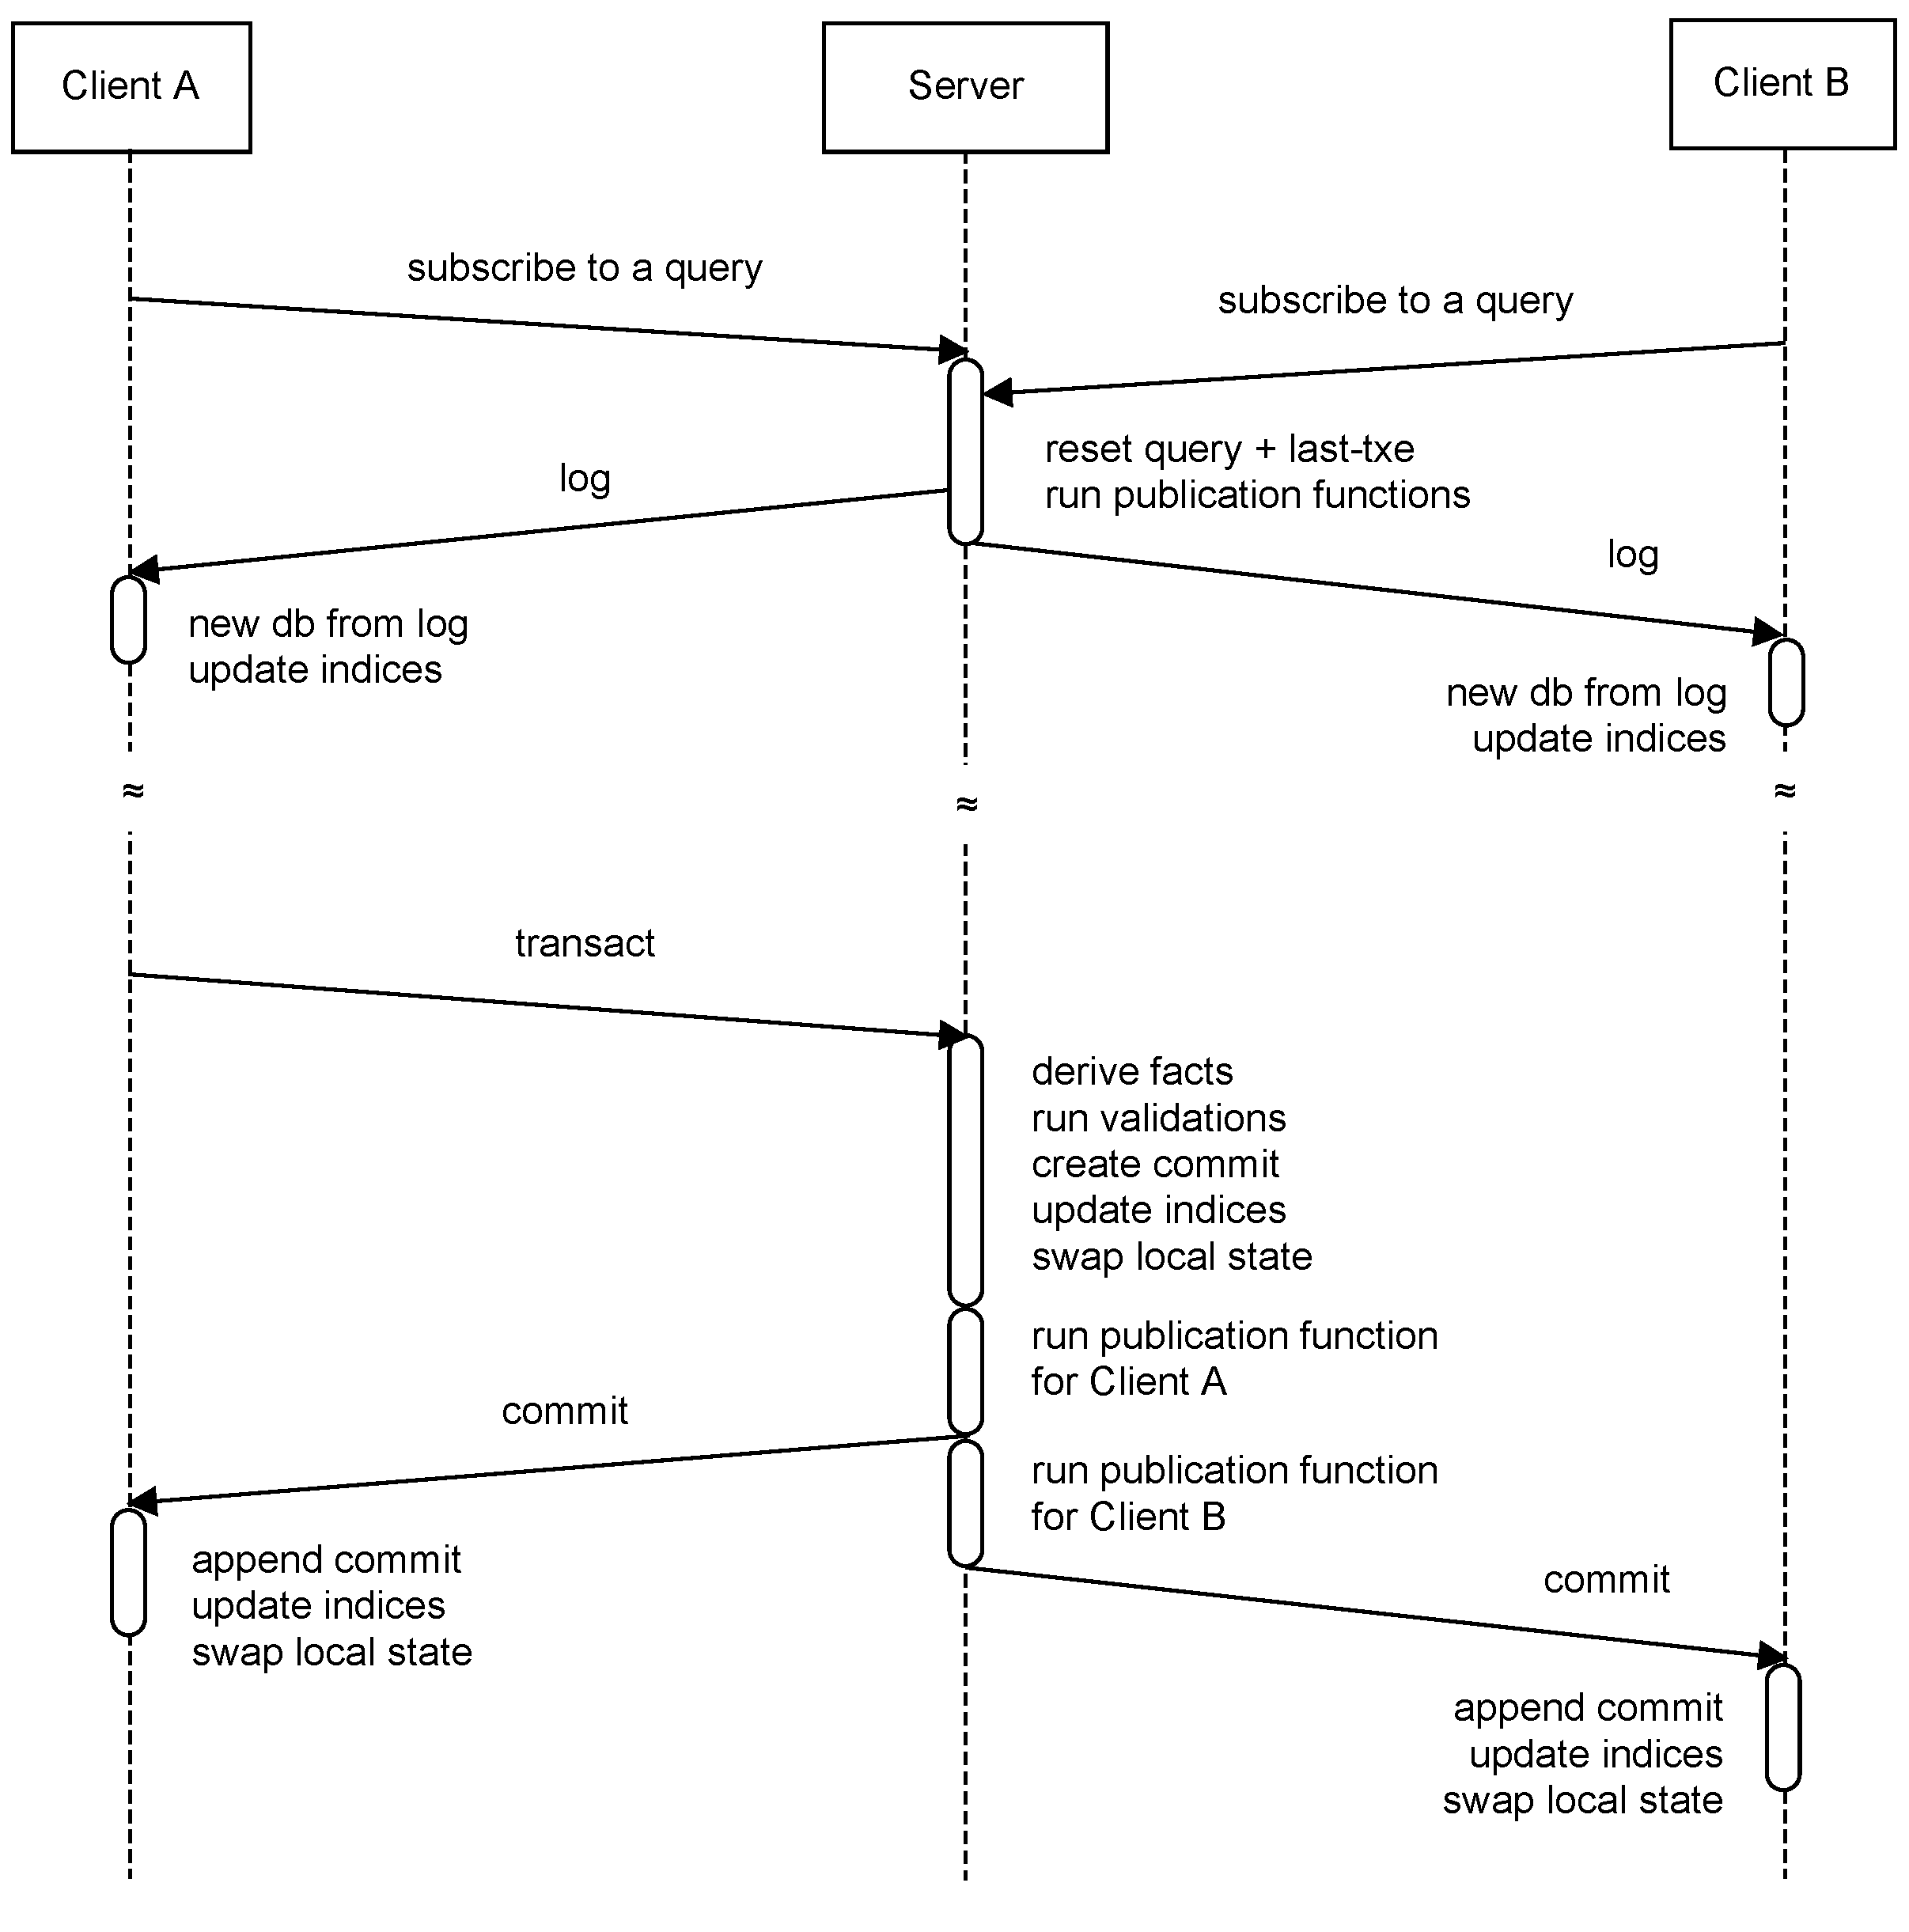
\includegraphics[width=\linewidth]{images/pubsub.pdf}
  \caption{Sequence diagram of subscription, transaction, and publication}
  \label{fig:pubsub}
\end{figure}



\paragraph{Nontrivial publications.}
The publication function may also modify facts, e.g. censor some values matching sensitive attributes or choose to not publish facts matching some pattern. As a consequence of the simplistic notification mechanism, the server may send more or less, or different facts than the client asked for. While the body of the publication function can be trivial and always return the latest commit regardless of query, developers building larger systems will likely need to put a lot of effort into writing an efficient, secure, and correct publication function. The simplistic design of the publication/subscription mechanism appears to be the weakest point of the presented data layer, as it only shifts to the developer almost all of the complexity related to efficiently distributing and diffing results from changed queries.

\cleardoublepage
\section{Discussion}\label{sec:discussion}

The following two subsections qualitatively review the contribution with respect to the stated goals, and expose limitations of the current implementation as well as discuss flaws inherent to the design.

\subsection{Advantages}

minimal loc shows expressive power of language

pluggable transport

free indexing

immutability and db-as-value

\paragraph{Flexible data model.} Representing data as fully-normalized fact triples allows

\paragraph{Auditability.} Accreting all facts in an immutable log gives complete auditability with no programmatic overhead.



\paragraph{}
In a traditional, row-oriented data model, modeling such data leads to wide, sparse tuples. Attribute-oriented data models can represent such data much more efficiently, and materialize only necessary attributes, at the cost of frequent multi-way joins across relations \cite{gobel2019optimising}.


\paragraph{Simple, yet useful bitemporality.}
problem: back dated changes. should we allow future dated changes? -- leaning towards no? or ignore? or cut off at "now" by default? we just defer answering this question as not a core concern of this poc

\paragraph{Library, not a framework.} Thinking of j

\paragraph{Easily extensible.} Customizing the behavior of the database is simple, as exemplified by the implementation of the \lisp{document} function which allows atomic ingestion of multiple facts related to an entity as arbitrarily nested documents. Another example would be the client side use of a single database to store both local \gls{UI} state and "global" facts from the server, the only change necessary is to filter out attributes with a \lisp{:local} namespace before transacting the change to the server.


\subsection{Limitations}


\paragraph{Datalog semantics.}


\paragraph{Query library.}

a dynamic that favours those building new systems as opposed to those that maintain or steward large existing systems.

\paragraph{Set vs. multiset semantics.}
-- determining if fact was superseded needs upfront specification of cardinality for field.
-- TODO does it make sense to default to cardinality one?
set vs multiset semantics -- leaning towards set on insertion, multiset on querying


\paragraph{No temporal constraints.} temporal and general constraints

\paragraph{Privacy regulations.} Excision

\paragraph{Access control.} what do do when roles change?

\paragraph{Latency compensation.} Optimistic updates

\paragraph{Safe abstraction and composition of queries.} Currently, the query engine provides no means for abstracting and composing fragments of queries (called "rules" in Datomic) in a \emph{hygienic} way, i.e. so that expected lexical scoping semantics of logic variables are observed.

\paragraph{Coupled storage.} The design of the storage layer currently makes no provisions for an offloading of responsibilities to a generic storage backend as in Datomic.

\paragraph{Coupled transactor.} Splitting out the transactor component as in Datomic, with the goal of increasing availability in a failover configuration, is not possible in the current design.

\paragraph{Explicit subscriptions.} Clients have to explicitly subscribe and manage the lifecycle of available publications, which requires duplicate, imperative, and error-prone programming effort.

\paragraph{Expensive re-indexing.} Whenever \emph{novelty} (assertions or retractions of facts) arrives, the index is rebuilt in a blocking fashion. The database should at least allow accumulation of \emph{some} novelty, and allow queries to leverage a combination of the (stale) sorted indices together with the linear accumulation of novelty to produce results before novelty is indexed.

\paragraph{No real bitemporal queries.} A complex query might want to mix different timelines in single query, e.g. join previous values with current values.

\paragraph{Incompatibility with proliferated standards.} Simultaneously changing the data model, its representation and storage formats, the interfaces and protocols, query languages and semantics requires doing away with

\paragraph{Switching costs.} Since persistence of data is fundamental to any application, changes to the data layer of existing systems are prohibitively expensive. Yet, the same dynamic proves advantageous in green field projects unencumbered by legacy decisions.

\paragraph{Open vs. closed system.} Incidental complexity within a closed system such as the one described in this work can be managed to stay at a minimal level because any outside components the system is interacting with is forced to adapt to the system's way. However, users of such a system eventually want to connect it to other things. Inevitably, doing so \emph{imports} some of the incidental complexities of those systems. It remains to be seen if we can build open systems without importing accidental complexity \cite{moffat16eve}.

\paragraph{Second system effect.} This work is the author's second attempt dealing with the problems of data layers for business applications. Brooks observed the tendency of successful systems to be succeeded by over-engineered, bloated systems, due to inflated expectations and overconfidence of the authors \cite{brooks1995mythical}.

\cleardoublepage
\section{Future Work}

\paragraph{Safe concurrent editing.}
A distributed system expects connection loss and simultaneous conflicting edits. It should be possible to define a schema that selects one of many built-in conflict resolution strategies specific to the domain requirements of each attribute. A per-field specifiable tradeoff as dictated by the \gls{cap} theorem of C and A must propagate to the clients and dictate the possible operations on the data item in question given the current network conditions \cite{emerick2014api}.


A \gls{DRP} approach by \cite{margara2014we} focuses strongly on selectable consistency guarantees, while \gls{CRDT} and \gls{OT} are recently discovered concepts which appear to provide composable consistency primitives for robust replication \cite{weilbach2015replikativ, weilbach2016decoupling}.

The Braid protocol \cite{braid19} is an in-progress draft of a proposed \gls{IETF} standard to add history, editing, and subscription semantics to HTTP resources. It aims to standardize the representation and synchronization of arbitrary web application state. Braid can allow simultaneous editing of the same resource by different clients and servers and can guarantee a consistent resulting state via selectable \emph{merge types} implementing various CRDTs and OTs.


\paragraph{(Temporal) logic constraints.} An ideal programming environment would let the programmer "use logic to express what is true, use logic to check whether something is true, [and] use logic to find out what is true \cite{sicp}". Research by \cite{alvaro2010dedalus,alvaro2011consistency} explores temporal extensions to Datalog and a domain-specific language for describing time-dependent behavior of distributed systems.

\paragraph{Full stack laziness.} A fully lazy distributed data structure would allow transparent access and local caching of all facts for which the client passes access rules set up by the server. Such a design would also allow transparent querying of past facts, possibly aided by hints from the programmer as to where (on client or server) the query should be executed.

\paragraph{Incremental maintenance.} Efficient execution of Datalog programs installed as "live" queries entails incremental updating of the result set as the source data changes.
Research in the direction of incremental view maintenance in such systems includes timely dataflow \cite{murray2013naiad}, differential dataflow \cite{mcsherry2013differential}, and 3DF providing an implementation of reactive Datalog for Datomic \cite{gobel2019optimising}.


\paragraph{Data as code.} As the presented system's flexibility allows storing, versioning, replicating and querying arbitrary data, including functions, the question arises of how an entire application can be constructed with all its code existing as facts inside the database, replicating to the clients -- thus closing the circle back to MUMPS-like systems.


\cleardoublepage
\section{Conclusion}


\renewcommand{\listtablename}{Tables}

\listoffigures
\begingroup
\let\clearpage\relax
\listoftables
\endgroup
\begingroup
\let\clearpage\relax
\lstlistoflistings
\endgroup


\bibliography{lit}
\bibliographystyle{alpha}

\end{document}
